% Created 2014-10-15 Wed 15:18
\documentclass[bigger]{beamer}
\usepackage[utf8]{inputenc}
\usepackage[T1]{fontenc}
\usepackage{fixltx2e}
\usepackage{graphicx}
\usepackage{longtable}
\usepackage{float}
\usepackage{wrapfig}
\usepackage{soul}
\usepackage{textcomp}
\usepackage{marvosym}
\usepackage{wasysym}
\usepackage{latexsym}
\usepackage{amssymb}
\usepackage{hyperref}
\tolerance=1000
\mode<beamer>{\usetheme[compress]{Berlin}}
\usepackage{graphicx}
\usepackage{amsmath}
\usepackage{lmodern}
\usepackage{ifmtarg}
\usepackage{multicol}
\usepackage{multirow}
\usepackage{tikz}
\usetikzlibrary{calc}
\usepackage{nth}
\makeatletter
\newcommand\ChangeItemFont[3]{%
\renewcommand{\itemize}[1][]{%
  \beamer@ifempty{##1}{}{\def\beamer@defaultospec{#1}}%
  \ifnum \@itemdepth >2\relax\@toodeep\else
    \advance\@itemdepth\@ne
    \beamer@computepref\@itemdepth% sets \beameritemnestingprefix
    \usebeamerfont{itemize/enumerate \beameritemnestingprefix body}%
    \usebeamercolor[fg]{itemize/enumerate \beameritemnestingprefix body}%
    \usebeamertemplate{itemize/enumerate \beameritemnestingprefix body begin}%
    \list
      {\usebeamertemplate{itemize \beameritemnestingprefix item}}
      {\def\makelabel####1{%
          {%
            \hss\llap{{%
                \usebeamerfont*{itemize \beameritemnestingprefix item}%
                \usebeamercolor[fg]{itemize \beameritemnestingprefix item}####1}}%
          }%
        }%
  \ifnum\@itemdepth=1\relax
    #1%
  \else
  \ifnum\@itemdepth=2\relax
    #2%
  \else
  \ifnum\@itemdepth=3\relax
    #3%
  \fi%
  \fi%
  \fi%
  }
  \fi%
  \beamer@cramped%
  \raggedright%
  \beamer@firstlineitemizeunskip%
}}
\makeatother

\setbeamertemplate{footline}
  {%
    \begin{beamercolorbox}[colsep=1.5pt]{upper separation line foot}
    \end{beamercolorbox}
    \begin{beamercolorbox}[ht=2.5ex,dp=1.125ex,%
      leftskip=.3cm,rightskip=.3cm plus1fil]{author in head/foot}%
      \leavevmode{\usebeamerfont{author in head/foot}\insertshortauthor}%
      \hfill%
      {\usebeamerfont{institute in head/foot}\usebeamercolor[fg]{institute in head/foot}\insertshortinstitute}%
    \end{beamercolorbox}%
    \begin{beamercolorbox}[ht=2.5ex,dp=1.125ex,%
      leftskip=.3cm,rightskip=.3cm plus1fil]{title in head/foot}%
      {\usebeamerfont{title in head/foot}\insertshorttitle}%
      \hfill%
      {\usebeamerfont{frame number}\usebeamercolor[fg]{frame number}\insertframenumber~/~\inserttotalframenumber}
    \end{beamercolorbox}%
    \begin{beamercolorbox}[colsep=1.5pt]{lower separation line foot}
    \end{beamercolorbox}
  }
\makeatother


%----------------------------------------------------------------------
% Define useful commands
%----------------------------------------------------------------------

\newcommand{\eejj}{\ensuremath{eejj} }
\newcommand{\enujj}{\ensuremath{e\nu jj} }
\newcommand{\mumujj}{\ensuremath{\mu\mu jj} }
\newcommand{\munujj}{\ensuremath{\mu\nu jj} }
\newcommand{\emujj}{\ensuremath{e\mu jj} }
\newcommand{\zjets}{\ensuremath{\text{Z}^{0}}+jets }
\newcommand{\wjets}{\ensuremath{\text{W}^{\pm}}+jets }
\newcommand{\ttbar}{\ensuremath{t\bar{t}} }

\newcommand{\pt}{\ensuremath{p_{\text{T}}} }
\newcommand{\ST}{\ensuremath{S_{\text{T}}} }
\newcommand{\mee}{\ensuremath{m_{\text{ee}}} }
\newcommand{\mll}{\ensuremath{m_{\ell\ell}} }
\newcommand{\mej}{\ensuremath{m_{\text{ej}}} }
\newcommand{\mejmin}{\ensuremath{m_{\text{ej}}^{\text{min}}} }
\newcommand{\mejavg}{\ensuremath{m_{\text{ej}}^{\text{avg}}} }
% \newcommand{\mt}{\ensuremath{m_{\text{T, e}\nu}}}
\newcommand{\mtjnu}{\ensuremath{m_{\text{T, j}\nu}} }


\newcommand{\met}{\ensuremath{\not\!\!{E_{\text{T}}}} }
\newcommand{\mt}{\ensuremath{m_{\text{T, e}\nu}} }

%----------------------------------------------------------------------
% Define useful numbers
%----------------------------------------------------------------------

% Lumi info
\newcommand{\intLumi}{$19.6 \text{ fb}^{-1}$}

% MC scale factors
\newcommand{\enujjWJetsMonteCarloScaleFactor}{0.85 \pm 0.01 \text{ (stat)} \pm 0.01    \text{ (syst)}}
\newcommand{\enujjTTBarMonteCarloScaleFactor}{0.97 \pm 0.02 \text{ (stat)} \pm 0.01    \text{ (syst)}}
% \newcommand{\eejjZJetsMonteCarloScaleFactor} {0.97 \pm 0.01 \text{ (stat)} \pm 0.00004 \text{ (syst)}}
\newcommand{\eejjZJetsMonteCarloScaleFactor} {0.97 \pm 0.01 \text{ (stat)}}

\newcommand{\enujjWJetsMonteCarloScaleFactorMETRescaled}{0.95 \pm 0.02 \text{ (stat)} \pm 0.01 \text{ (syst)}}
\newcommand{\enujjTTBarMonteCarloScaleFactorMETRescaled}{1.07 \pm 0.03 \text{ (stat)} \pm 0.01 \text{ (syst)}}

\newcommand{\enujjWJetsMonteCarloScaleFactorMETandMTRescaled}{0.97 \pm 0.02 \text{ (stat)} \pm 0.01 \text{ (syst)}}
\newcommand{\enujjTTBarMonteCarloScaleFactorMETandMTRescaled}{1.08 \pm 0.03 \text{ (stat)} \pm 0.01 \text{ (syst)}}

\newcommand{\eejjZControlRegionContamination}{4\%}

% Electron scale factors
\newcommand{\electronRecoDataMCScaleFactor}{0.98}
\newcommand{\electronRecoDataMCScaleFactorRelUnc}{1.5}
\newcommand{\electronRecoDataMCScaleFactorSqr}{0.96}

% GEN-level cross-sections (not yet rescaled) 
\newcommand{\wjetsXSection}{37509.0 pb}
\newcommand{\zjetsXSection}{3503.71 pb}
\newcommand{\ttbarXSection}{234 pb}
\newcommand{\stopSChannelXSection}{5.55 pb}
\newcommand{\stopTChannelXSection}{87.1 pb}
\newcommand{\stopTWChannelXSection}{22.2 pb}
\newcommand{\wwXSection}{57.1 pb} % THESE NEED TO BE UPDATED!!!
\newcommand{\wzXSection}{32.3 pb} % THESE NEED TO BE UPDATED!!!
\newcommand{\zzXSection}{8.26 pb} % THESE NEED TO BE UPDATED!!!

% QCD contributions at limit of the analysis
\newcommand{\percentQCDatEEJJLimit}{1\%}
\newcommand{\percentQCDatENuJJLimit}{3\%}

% Closure test contamination
\newcommand{\percentContaminationClosureTest}{5\%}
\newcommand{\percentContaminationClosureTestFinal}{55\%}

% Closure test (low-ST) results
\newcommand{\closureTestLowSTPredicted}{13100}
\newcommand{\closureTestLowSTPredictedUnc}{400}
\newcommand{\closureTestLowSTObserved}{12100}
\newcommand{\closureTestLowSTObservedUnc}{400}
\newcommand{\closureTestLowSTRatio}{1.08}
\newcommand{\closureTestLowSTRatioUnc}{0.05}

% Closure test (mid-ST) results
\newcommand{\closureTestMidSTPredicted}{877}
\newcommand{\closureTestMidSTPredictedUnc}{46.7}
\newcommand{\closureTestMidSTObserved}{600}
\newcommand{\closureTestMidSTObservedUnc}{53}
\newcommand{\closureTestMidSTRatio}{1.46}
\newcommand{\closureTestMidSTRatioUnc}{0.15}

% QCD systematic uncertainty
\newcommand{\qcdSystematicUncertaintyPerEle}{30\%}
\newcommand{\qcdSystematicUncertaintyTwoEle}{60\%}

% TTbar (e-mu-jj) contamination
\newcommand{\emujjContamination}{2\%}
\newcommand{\emujjRecoScaleFactor}{0.974  \pm 0.011 \text{ (stat)}}

% mumujj/munujj scale factors for data-driven background
\newcommand{\mumujjRecoScaleFactor}{97.5 \pm 0.4 \text{ (stat)}}
\newcommand{\munujjRecoScaleFactor}{97.2 \pm 0.5 \text{ (stat)}}

% Shape uncertainties
\newcommand{\enujjWJetsShapeUncertainty}{5.92\%}
\newcommand{\enujjTTBarShapeUncertainty}{8.17\%}
\newcommand{\eejjZJetsShapeUncertainty}{8.70\%}

% EES uncertainties
\newcommand{\electronEnergyScaleUncBarrel}{0.4\%}
\newcommand{\electronEnergyScaleUncEndcap}{4.1\%}

% EER uncertainties
\newcommand{\electronEnergyResolutionUncBarrel}{1.006}
\newcommand{\electronEnergyResolutionUncEndcap}{1.015}

% lumi uncertainty
\newcommand{\lumiUncertainty}{2.6\%}

% limits
\newcommand{\eejjObservedLimit}{1005}
\newcommand{\eejjExpectedLimit}{1030}
\newcommand{\enujjObservedLimit}{845}
\newcommand{\enujjExpectedLimit}{890}

\newcommand{\enujjObservedLimitCombined}{845}
\newcommand{\enujjExpectedLimitCombined}{932}

\newcommand{\eejjObservedLimitNoSyst}{1010}
\newcommand{\eejjExpectedLimitNoSyst}{1030}
\newcommand{\enujjObservedLimitNoSyst}{850}
\newcommand{\enujjExpectedLimitNoSyst}{895}

\newcommand{\eejjObservedLimitMuon}{1015}
\newcommand{\eejjExpectedLimitMuon}{980}
\newcommand{\enujjObservedLimitMuon}{825}
\newcommand{\enujjExpectedLimitMuon}{890}


\newcommand{\lowBetaExpectedLimit}{790}
\newcommand{\lowBetaObservedLimit}{635}

\mode<beamer>{\usecolortheme{bear}}
\mode<beamer>{\titlegraphic{\includegraphics[width=0.2\textwidth]{brown-logo}}}
\institute[Brown University]{\inst{1} Brown University \and \inst{2} University of Alabama \and \inst{3} Rome}
\providecommand{\alert}[1]{\textbf{#1}}

\title{Search for Leptoquarks at CMS}
\author{Edmund Berry}
\date{Wednesday, October 15, 2014}
\hypersetup{
  pdfkeywords={},
  pdfsubject={},
  pdfcreator={Emacs Org-mode version 7.9.3f}}

\author[Edmund Berry]{\alert{E. Berry}\inst{1}, S. Cooper\inst{2}, P. Rumerio\inst{2}, F. Santanastasio\inst{3}}
\begin{document}

\maketitle


\section{Introduction}
\label{sec-1}
\subsection{Theory}
\label{sec-1-1}
\begin{frame}
\frametitle{Leptons and quarks}
\label{sec-1-1-1}
%% Table
\label{sec-1-1-1-1}

\resizebox{\textwidth}{!}{
\begin{tabular}{c|ccc|cc|c|c}
    \multirow{2}{*}{Fermion type} & \multicolumn{3}{c|}{Generation} & \multirow{2}{*}{$T$} & \multirow{2}{*}{$T_3$} & \multirow{2}{*}{$Y$} & \multirow{2}{*}{$Q$} \\
    & \nth{1} & \nth{2} & \nth{3} & & & & \\
    \hline \hline
    \multirow{2}{*}{Leptons} & $\doublet{\nu_e}{e}_{L}$ & $\doublet{\nu_\mu}{\mu}_{L}$ & $\doublet{\nu_\tau}{\tau}_{L}$  & $\frac{1}{2}$ & $\doublet{\frac{1}{2}}{-\frac{1}{2}}$ & $-1$ & $\doublet {0}{-1}$ \\
    & $e_{R}$ & $\mu_{R}$ & $\tau_{R}$ & $0$ & $0$ & $-2$ & $-1$  \\
    \hline
    \multirow{3}{*}{Quarks} & $\doublet{u}{d}_{L}$ & $\doublet{c}{s}_{L}$ & $\doublet{t}{b}_{L}$ & $\frac{1}{2}$ & $\doublet{\frac{1}{2}}{-\frac{1}{2}}$ & $\frac{1}{3}$ & $\doublet {\frac{2}{3}}{-\frac{1}{3}}$ \\
    & $u_{R}$ & $c_{R}$ & $t_{R}$ & $0$ & $0$ & $\frac{4}{3}$ & $\frac{2}{3}$  \\
    & $d_{R}$ & $s_{R}$ & $b_{R}$ & $0$ & $0$ & $-\frac{2}{3}$ & $-\frac{1}{3}$ \\
  \end{tabular}
}
\begin{itemize}

\item Leptons and quarks are formally independent, but\ldots{}
\label{sec-1-1-1-2}%

\item Both come in three generations
\label{sec-1-1-1-3}%

\item Both have similar arrangement under EW interaction
\label{sec-1-1-1-4}%

\item Possible motivation: hypothetical interaction between leptons and quarks
\label{sec-1-1-1-5}%
\end{itemize} % ends low level
\end{frame}
\begin{frame}
\frametitle{Leptoquarks}
\label{sec-1-1-2}
\begin{columns}
\begin{column}{0.6\textwidth}
%% Text
\label{sec-1-1-2-1}

\footnotesize
\begin{itemize}
\item Search for a scalar boson carrying both baryon and lepton number and fractional charge
\item Leptoquark searches are traditionally grouped into generations
\item This search is for pair-production of \alert{first} generation leptoquarks
\item $\beta = \text{BR}(\text{LQ} \rightarrow e^{\pm}q)$ is treated as a free parameter,
leading to two separate analyses:
\begin{itemize}
\item \eejj: opt. for $\beta = 1.0$
\item \enujj: opt. for $\beta = 0.5$
\end{itemize}
\end{itemize}
\normalsize
\end{column}
\begin{column}{0.5\textwidth}
%% Figures
\label{sec-1-1-2-2}
%% eejj figure
\label{sec-1-1-2-2-1}

\centering
\eejj final state
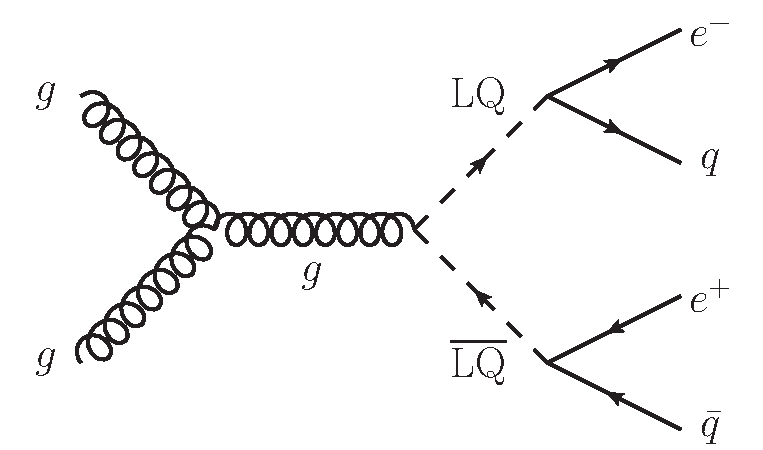
\includegraphics[width=0.8\textwidth]{fig/feynman/LQ_pair_decay_eejj.pdf}
%% enujj figure
\label{sec-1-1-2-2-2}

\centering
\enujj final state
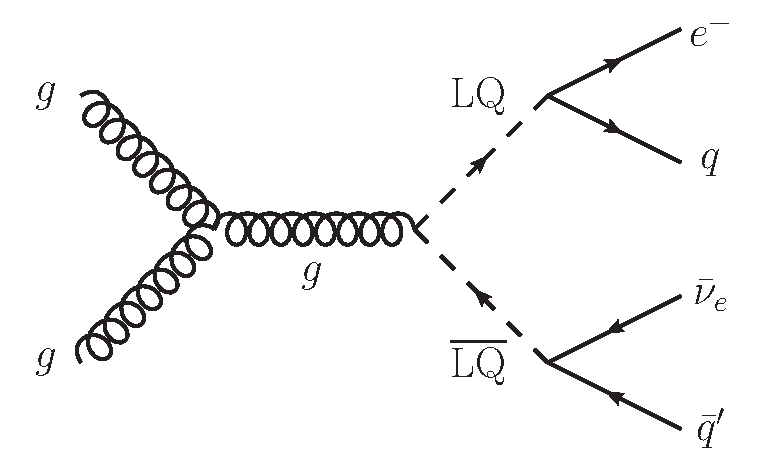
\includegraphics[width=0.8\textwidth]{fig/feynman/LQ_pair_decay_enujj.pdf}
\end{column}
\end{columns}
\end{frame}
\subsection{Strategy}
\label{sec-1-2}
\begin{frame}
\frametitle{Analysis strategy}
\label{sec-1-2-1}

\begin{itemize}
\item Define SM-dominated preselection for each analysis
\item Optimize final selection using $S/\sqrt{S+B}$
\begin{itemize}
\item Optimize a different selection for each LQ mass
\end{itemize}
\item For \eejj ($\beta = 1.0$) analysis, optimize cuts on:
\begin{itemize}
\item $\ST = \pt(e_1) + \pt(e_2) + \pt(j_1) + \pt(j_2)$
\item \mejmin
\item \mee
\end{itemize}
\item For \enujj ($\beta = 0.5$) analysis, optimize cuts on:
\begin{itemize}
\item $\ST = \pt(e) + \met + \pt(j_1) + \pt(j_2)$
\item \mej
\item \mt
\item \met
\end{itemize}
\item Set limit in plane of $M_{LQ}$ vs. $\beta$
\end{itemize}
\end{frame}
\section{\eejj analysis}
\label{sec-2}
\subsection{\eejj preselection}
\label{sec-2-1}
\begin{frame}
\frametitle{\eejj preselection definition}
\label{sec-2-1-1}
%% Notes
\label{sec-2-1-1-1}

\begin{itemize}
\item Exactly two electrons: $\pt > 45$ GeV and  $|\eta| < 2.5$
\item At least two jets
\item $\pt(j_1) > 125$ GeV and $|\eta| < 2.4$
\item $\pt(j_2) > 45$ GeV and $|\eta| < 2.4$
\item $\mee > 50$ GeV
\item $\ST = \pt(e_1) + \pt(e_2) + \pt(j_1) + \pt(j_2) > 300$ GeV
\item Muon veto
\item Trigger with one electron + two jets
\end{itemize}
\end{frame}
\begin{frame}
\frametitle{\eejj preselection: \ST and \mej}
\label{sec-2-1-2}
\begin{columns}
\begin{column}{0.6\textwidth}
%% ST
\label{sec-2-1-2-1}

\centering
$\ST$
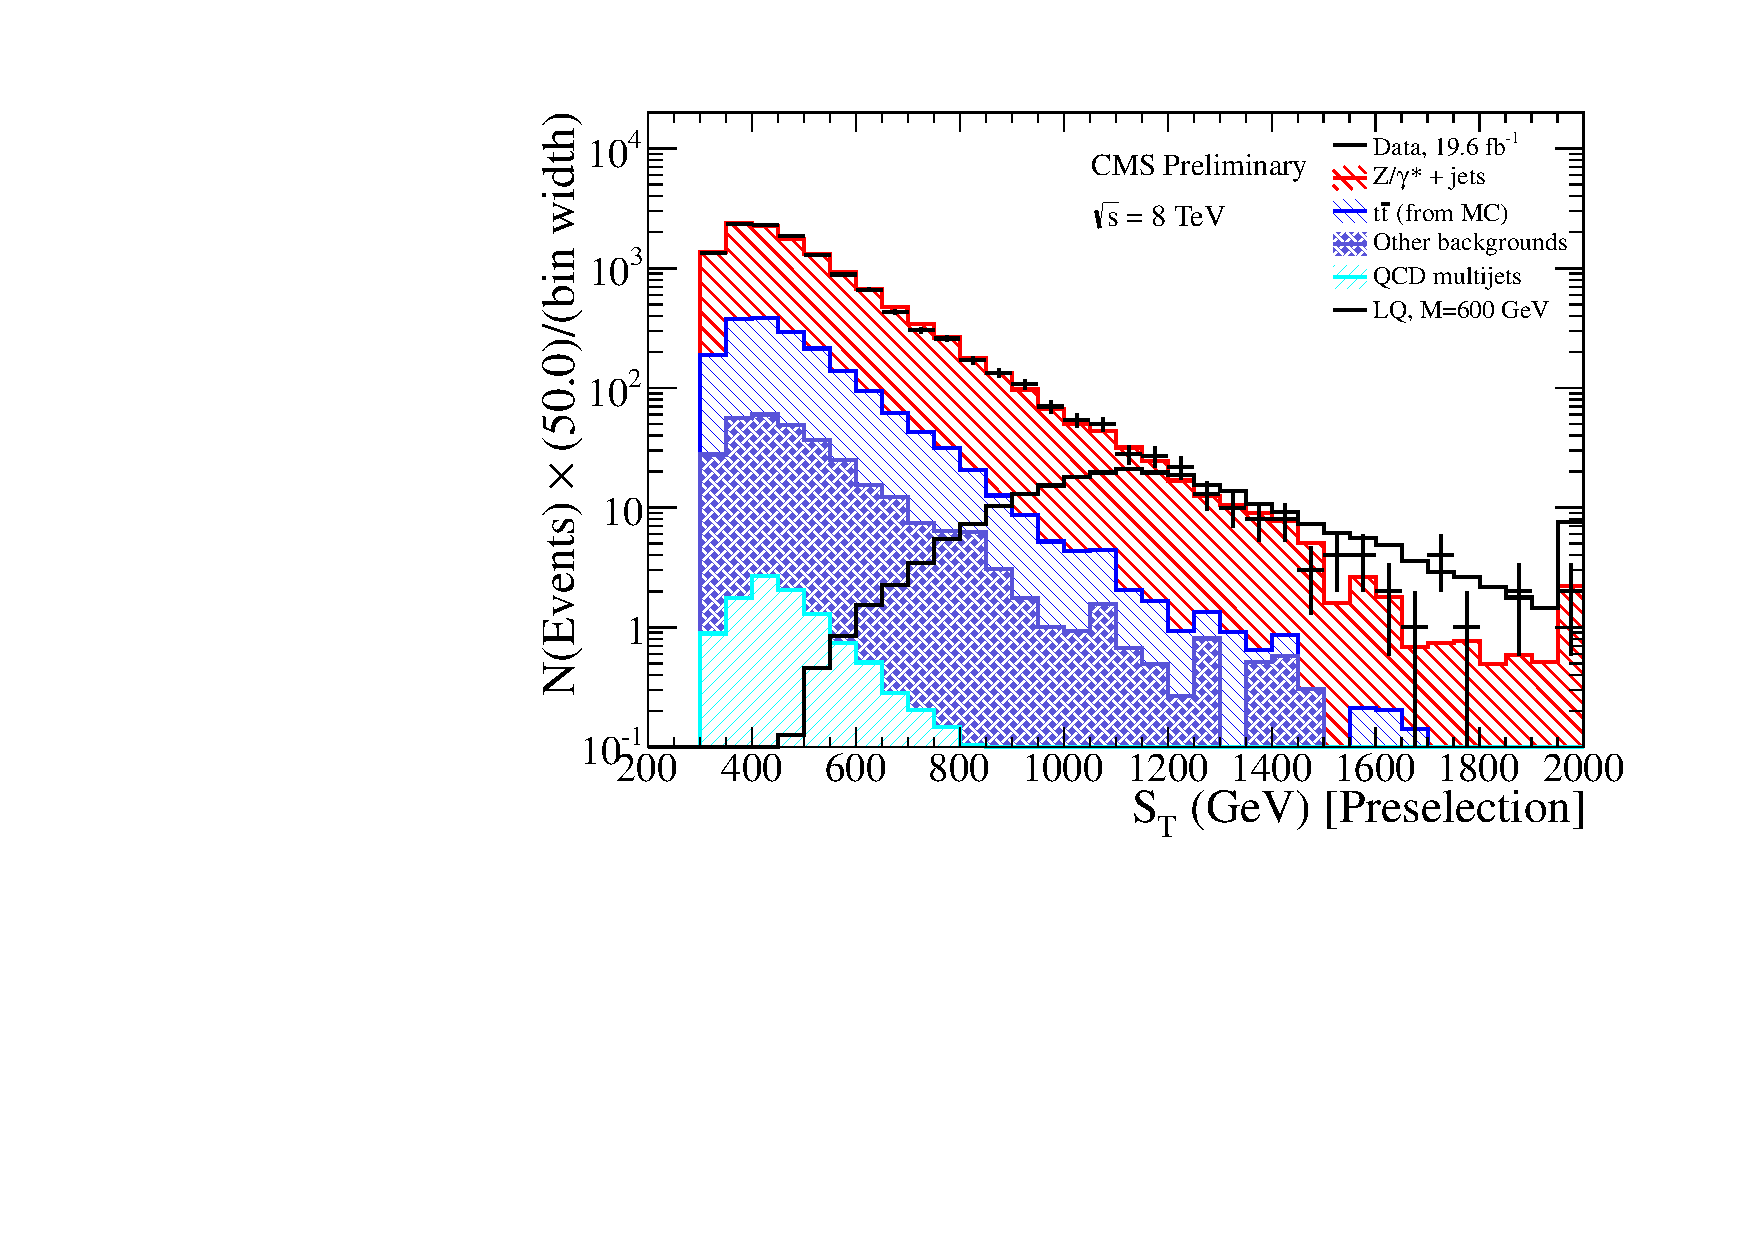
\includegraphics[width=\textwidth]{fig/ee/preselection_noRatio/sT_PAS_eejj.pdf}
\end{column}
\begin{column}{0.6\textwidth}
%% MEJ
\label{sec-2-1-2-2}

\centering
\mej
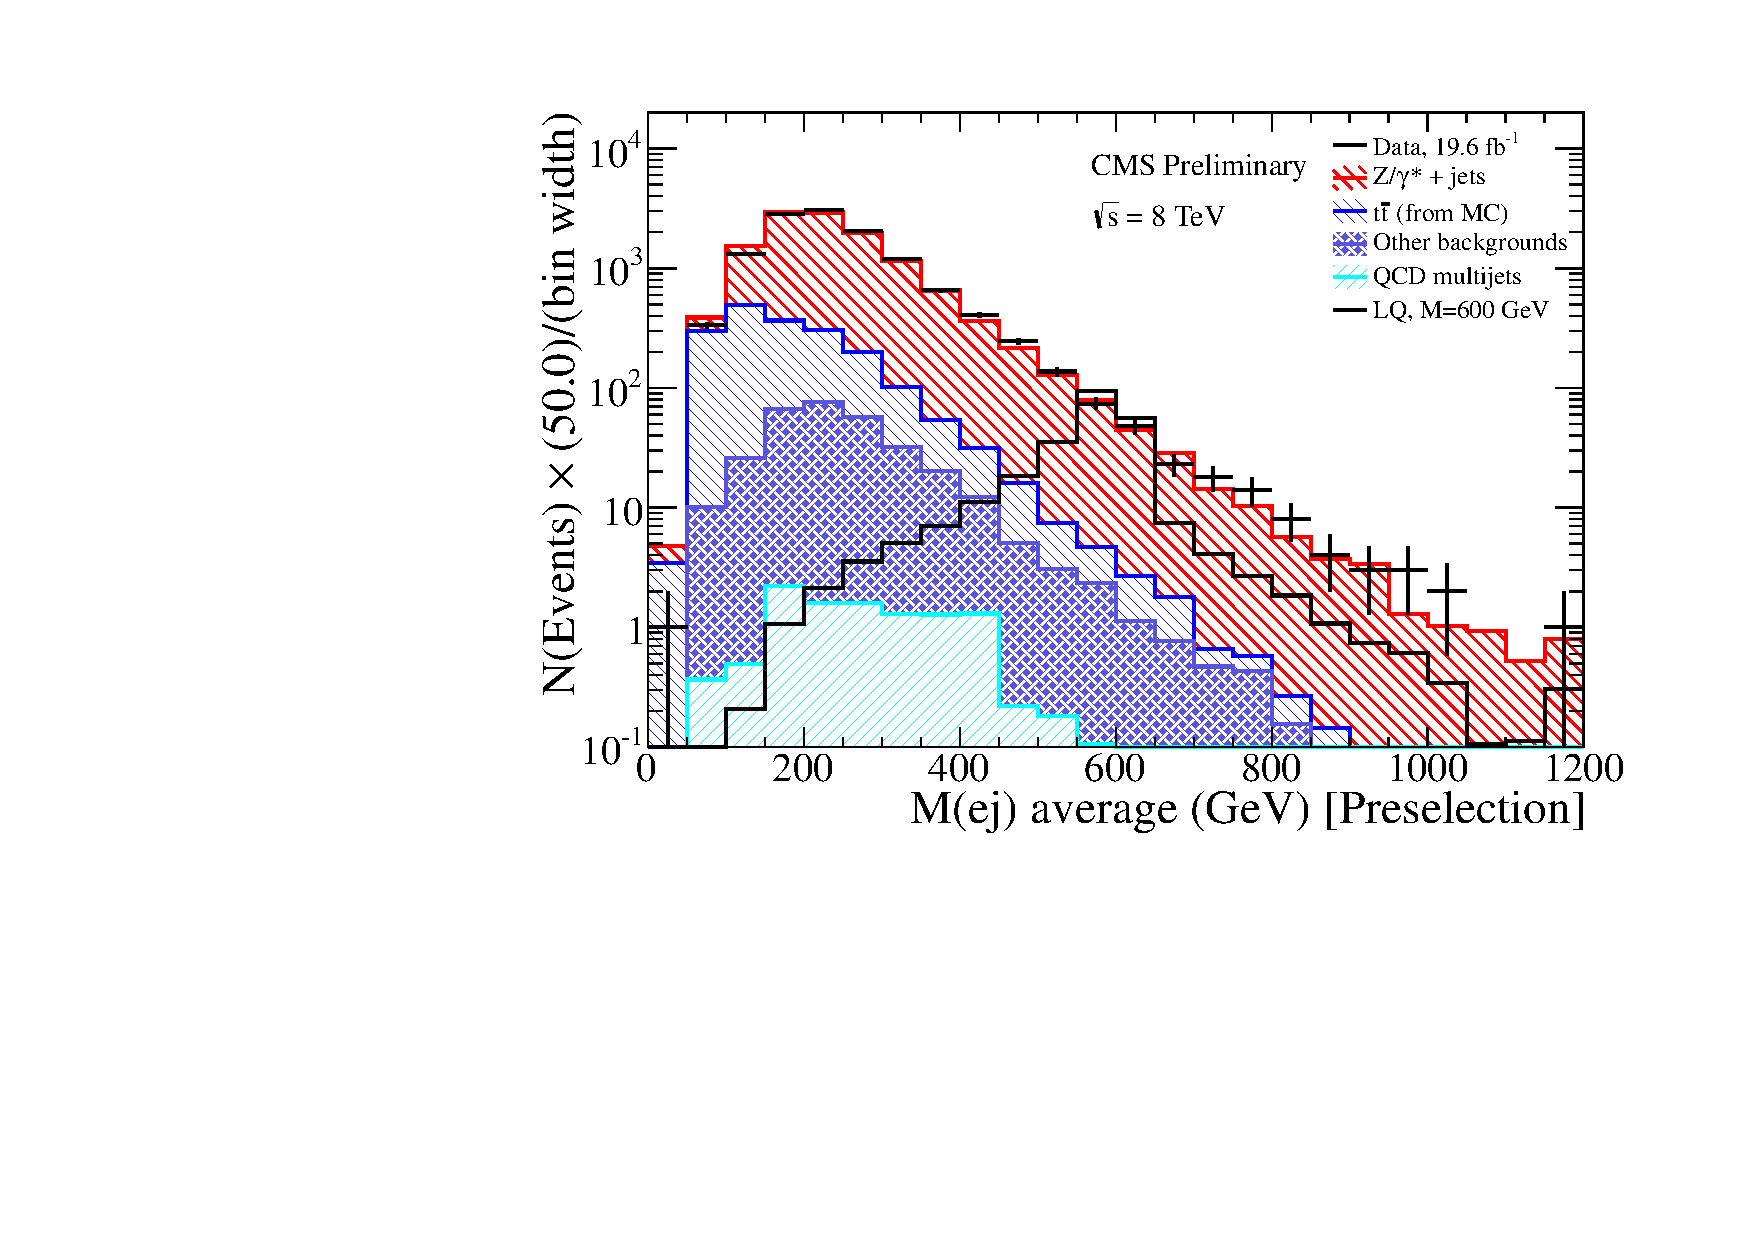
\includegraphics[width=\textwidth]{fig/ee/preselection_noRatio/Mej_selected_avg_PAS_eejj.pdf}
\end{column}
\end{columns}
\end{frame}
\subsection{\eejj backgrounds}
\label{sec-2-2}
\begin{frame}
\frametitle{\eejj backgrounds}
\label{sec-2-2-1}
\begin{block}{Backgrounds include:}
\label{sec-2-2-1-1}
\begin{itemize}

\item \zjets: shape from MC, normalization from data \\ (dominant background)
\label{sec-2-2-1-1-1}%

\item \ttbar: shape and normalization from data
\label{sec-2-2-1-1-2}%

\item QCD multijets: shape and normalization from data
\label{sec-2-2-1-1-3}%

\item Other backgrounds: shape and normalization from MC
\label{sec-2-2-1-1-4}%
\end{itemize} % ends low level
\end{block}
\end{frame}
\subsection{\eejj optimization}
\label{sec-2-3}
\begin{frame}
\frametitle{\eejj final selection optimization table}
\label{sec-2-3-1}
%% Text
\label{sec-2-3-1-1}

\begin{itemize}
\item Optimize \ST, \mejmin, \mee after \eejj preselection
\begin{itemize}
\item $e$-$j$ pairs are chosen to minimize the difference between the mass of each pair
\item \mejmin is the smallest of the two mass pairs
\end{itemize}
\item Optimization figure of merit is $S/\sqrt{S+B}$
\item Results:
\end{itemize}
%% Table
\label{sec-2-3-1-2}

\resizebox{\textwidth}{!}{
\begin{tabular}{l|c|c|c|c|c|c|c|c|c|c|c|c|c|c|c|}
\cline{2-16} 
& \multicolumn{15}{c|}{LQ mass (\eejj)} \\ 
\cline{2-16} 
& 300 & 350 & 400 & 450 & 500 & 550 & 600 & 650 & 700 & 750 & 800 & 850 & 900 & 950 & $\geq 1000$ \\
\hline 
\hline 
\multicolumn{1}{|c|}{\ST [GeV]}  & 435 & 485 & 535 & 595 & 650 & 715 & 780 & 850 & 920 & 1000 & 1075 & 1160 & 1245 & 1330 & 1425 \\
\multicolumn{1}{|c|}{\mee [GeV]}  & 110 & 110 & 115 & 125 & 130 & 140 & 145 & 155 & 160 & 170 & 175 & 180 & 190 & 195 & 205 \\
\multicolumn{1}{|c|}{\mejmin [GeV]}  & 50 & 105 & 160 & 205 & 250 & 290 & 325 & 360 & 390 & 415 & 435 & 450 & 465 & 470 & 475 \\
\hline 
\hline 
\end{tabular}
}%
\end{frame}
\subsection{\eejj final selection}
\label{sec-2-4}
\begin{frame}
\frametitle{\eejj final selection table}
\label{sec-2-4-1}
%% Table
\label{sec-2-4-1-1}

\resizebox{\textwidth}{!}{
\begin{tikzpicture}
\node (table) {
\begin{tabular}{| l | c | c | c | c | c | c | c | c |} 
\hline 
$M_{LQ}$ & LQ Signal & Z+Jets & $t\bar{t}$ (from data) & QCD (from data) & Other & Data &  Total Background & Significance\\ 
\hline 
\hline 
Presel & - &  $ 10538.4 \pm 35.8 $ & $ 1566.6 \pm 29.2 $ & $ 10.87 \pm 0.10 $ & $ 303.8 \pm 7.4 $ &12442 & $ 12419.6 \pm 46.8 $ & NA \\ 
\hline 
300 &  $ 13560.2\pm 80.1 $ &  $ 462.2 \pm 7.4 $ & $ 724.3 \pm 19.8 $ & $ 5.282 \pm 0.052 $ & $ 62.1 \pm 4.6 $ & 1244 &  $ 1253.94 \pm 21.67 $ $ \pm $ $ 30.08 $ (syst) & 0.0 \\ 
350 &  $ 6473.9\pm 33.3 $ &  $ 332.1 \pm 6.2 $ & $ 352.0 \pm 13.8 $ & $ 3.215 \pm 0.036 $ & $ 37.7 \pm 3.6 $ & 736 &  $ 725.10 \pm 15.57 $ $ \pm $ $ 24.99 $ (syst) & 0.0 \\ 
400 &  $ 3089.3\pm 15.0 $ &  $ 203.2 \pm 4.8 $ & $ 153.7 \pm 9.1 $ & $ 1.696 \pm 0.023 $ & $ 23.8 \pm 2.9 $ & 389 &  $ 382.40 \pm 10.72 $ $ \pm $ $ 15.00 $ (syst) & 0.0 \\ 
450 &  $ 1508.1\pm 7.2 $ &  $ 112.9 \pm 3.5 $ & $ 86.9 \pm 6.9 $ & $ 0.890 \pm 0.016 $ & $ 11.8 \pm 2.0 $ & 233 &  $ 212.44 \pm 7.99 $ $ \pm $ $ 13.33 $ (syst) &  0.0 \\ 
500 &  $ 767.4\pm 3.6 $ &  $ 66.5 \pm 2.7 $ & $ 47.2 \pm 5.1 $ & $ 0.485 \pm 0.011 $ & $ 7.4 \pm 1.6 $ & 148 &  $ 121.61 \pm 5.96 $ $ \pm $ $ 6.03 $ (syst) &  1.8 \\ 
550 &  $ 410.5\pm 1.9 $ &  $ 37.4 \pm 2.1 $ & $ 25.8 \pm 3.7 $ & $ 0.2758 \pm 0.0084 $ & $ 3.7 \pm 1.1 $ & 81 &  $ 67.24 \pm 4.40 $ $ \pm $ $ 3.39 $ (syst) & 0.7 \\ 
600 &  $ 225.7\pm 1.0 $ &  $ 22.2 \pm 1.6 $ & $ 14.2 \pm 2.8 $ & $ 0.1527 \pm 0.0065 $ & $ 3.12 \pm 1.00 $ & 57 &  $ 39.66 \pm 3.35 $ $ \pm $ $ 2.42 $ (syst) & 2.1 \\ 
650 &  $ 125.85\pm 0.58 $ &  $ 14.0 \pm 1.2 $ & $ 5.4 \pm 1.7 $ & $ 0.0760 \pm 0.0040 $ & $ 1.05 \pm 0.47 $ & 36 &  $ 20.49 \pm 2.14 $ $ \pm $ $ 2.45 $ (syst) & 2.4 \\ 
700 &  $ 72.88\pm 0.33 $ &  $ 8.16 \pm 0.93 $ & $ 4.3 \pm 1.5 $ & $ 0.0448 \pm 0.0029 $ & $ 0.21 \pm 0.12 $ & 17 &  $ 12.74 \pm 1.80 $ $ \pm $ $ 2.15 $ (syst) & 0.9 \\ 
750 &  $ 43.10\pm 0.20 $ &  $ 4.88 \pm 0.69 $ & $ 1.55 \pm 0.90 $ & $ 0.0258 \pm 0.0023 $ & $ 0.078 \pm 0.038 $ & 12 &  $ 6.53 \pm 1.13 $ $ \pm $ $ 1.09 $ (syst) & 1.6 \\ 
800 &  $ 26.17\pm 0.12 $ &  $ 2.93 \pm 0.52 $ & $ 1.04 \pm 0.73 $ & $ 0.0193 \pm 0.0022 $ & $ 0.078 \pm 0.038 $ & 7 &  $ 4.06 \pm 0.90 $ $ \pm $ $ 0.89 $ (syst) & 1.1 \\ 
850 &  $ 15.978\pm 0.072 $ &  $ 2.34 \pm 0.48 $ & $ 0.52 \pm 0.52 $ & $ 0.0111 \pm 0.0015 $ & $ 0.042 \pm 0.028 $ & 5 &  $ 2.91 \pm 0.71 $ $ \pm $ $ 0.71 $ (syst) & 0.0\\ 
900 &  $ 9.813\pm 0.044 $ &  $ 1.23 \pm 0.36 $ & $ 0.52 \pm 0.52 $ & $ 0.0069 \pm 0.0012 $ & $ 0.022 \pm 0.020 $ & 3 &  $ 1.77 \pm 0.63 $ $ \pm $ $ 0.37 $ (syst) & 0.0 \\ 
950 &  $ 6.086\pm 0.028 $ &  $ 0.89 \pm 0.29 $ & $ 0.00_{-0.00}^{+1.14}$ &  $ 0.00451 \pm 0.00085 $ & $ 0.022 \pm 0.020 $ & 1 &  $ 0.912_{-0.295}^{+1.178}$ $ \pm $ $ 0.27 $ (syst) & 0.0 \\ 
1000 &  $ 3.860\pm 0.018 $ &  $ 0.56 \pm 0.22 $ & $ 0.00_{-0.00}^{+1.14}$ &  $ 0.00374 \pm 0.00082 $ & $ 0.0025 \pm 0.0025 $ & 1 &  $ 0.567_{-0.223}^{+1.162}$ $ \pm $ $ 0.17 $ (syst) & 0.0 \\ 
1050 &  $ 2.576\pm 0.011 $ &  $ 0.56 \pm 0.22 $ & $ 0.00_{-0.00}^{+1.14}$ &  $ 0.00374 \pm 0.00082 $ & $ 0.0025 \pm 0.0025 $ & 1 &  $ 0.567_{-0.223}^{+1.162}$ $ \pm $ $ 0.17 $ (syst) & 0.0 \\ 
1100 &  $ 1.6936\pm 0.0072 $ &  $ 0.56 \pm 0.22 $ & $ 0.00_{-0.00}^{+1.14}$ &  $ 0.00374 \pm 0.00082 $ & $ 0.0025 \pm 0.0025 $ & 1 &  $ 0.567_{-0.223}^{+1.162}$ $ \pm $ $ 0.17 $ (syst) & 0.0 \\ 
1150 &  $ 1.1272\pm 0.0047 $ &  $ 0.56 \pm 0.22 $ & $ 0.00_{-0.00}^{+1.14}$ &  $ 0.00374 \pm 0.00082 $ & $ 0.0025 \pm 0.0025 $ & 1 &  $ 0.567_{-0.223}^{+1.162}$ $ \pm $ $ 0.17 $ (syst) & 0.0 \\ 
1200 &  $ 0.7498\pm 0.0030 $ &  $ 0.56 \pm 0.22 $ & $ 0.00_{-0.00}^{+1.14}$ &  $ 0.00374 \pm 0.00082 $ & $ 0.0025 \pm 0.0025 $ & 1 &  $ 0.567_{-0.223}^{+1.162}$ $ \pm $ $ 0.17 $ (syst) & 0.0 \\ 
\hline
\end{tabular}
};
\draw [red,ultra thick,rounded corners]
($(table.south west) !.52! (table.north west)$)
rectangle 
($(table.south east) !.57! (table.north east)$);    
\draw [red,ultra thick,rounded corners]
($(table.north east) !.365! (table.north west)$)
rectangle 
($(table.south east) !0.! (table.north west)$);    
\end{tikzpicture}
}
%% Text
\label{sec-2-4-1-2}

\begin{itemize}
\item Broad excess of data w.r.t. total background
\item Most significant for $M_{\text{LQ}} = 650$ GeV selection
\end{itemize}
\end{frame}
\begin{frame}
\frametitle{\eejj final selection (650): \ST and \mejmin ($\beta = 1.0$)}
\label{sec-2-4-2}
\begin{columns}
\begin{column}{0.6\textwidth}
%% ST
\label{sec-2-4-2-1}

\centering
$\ST$
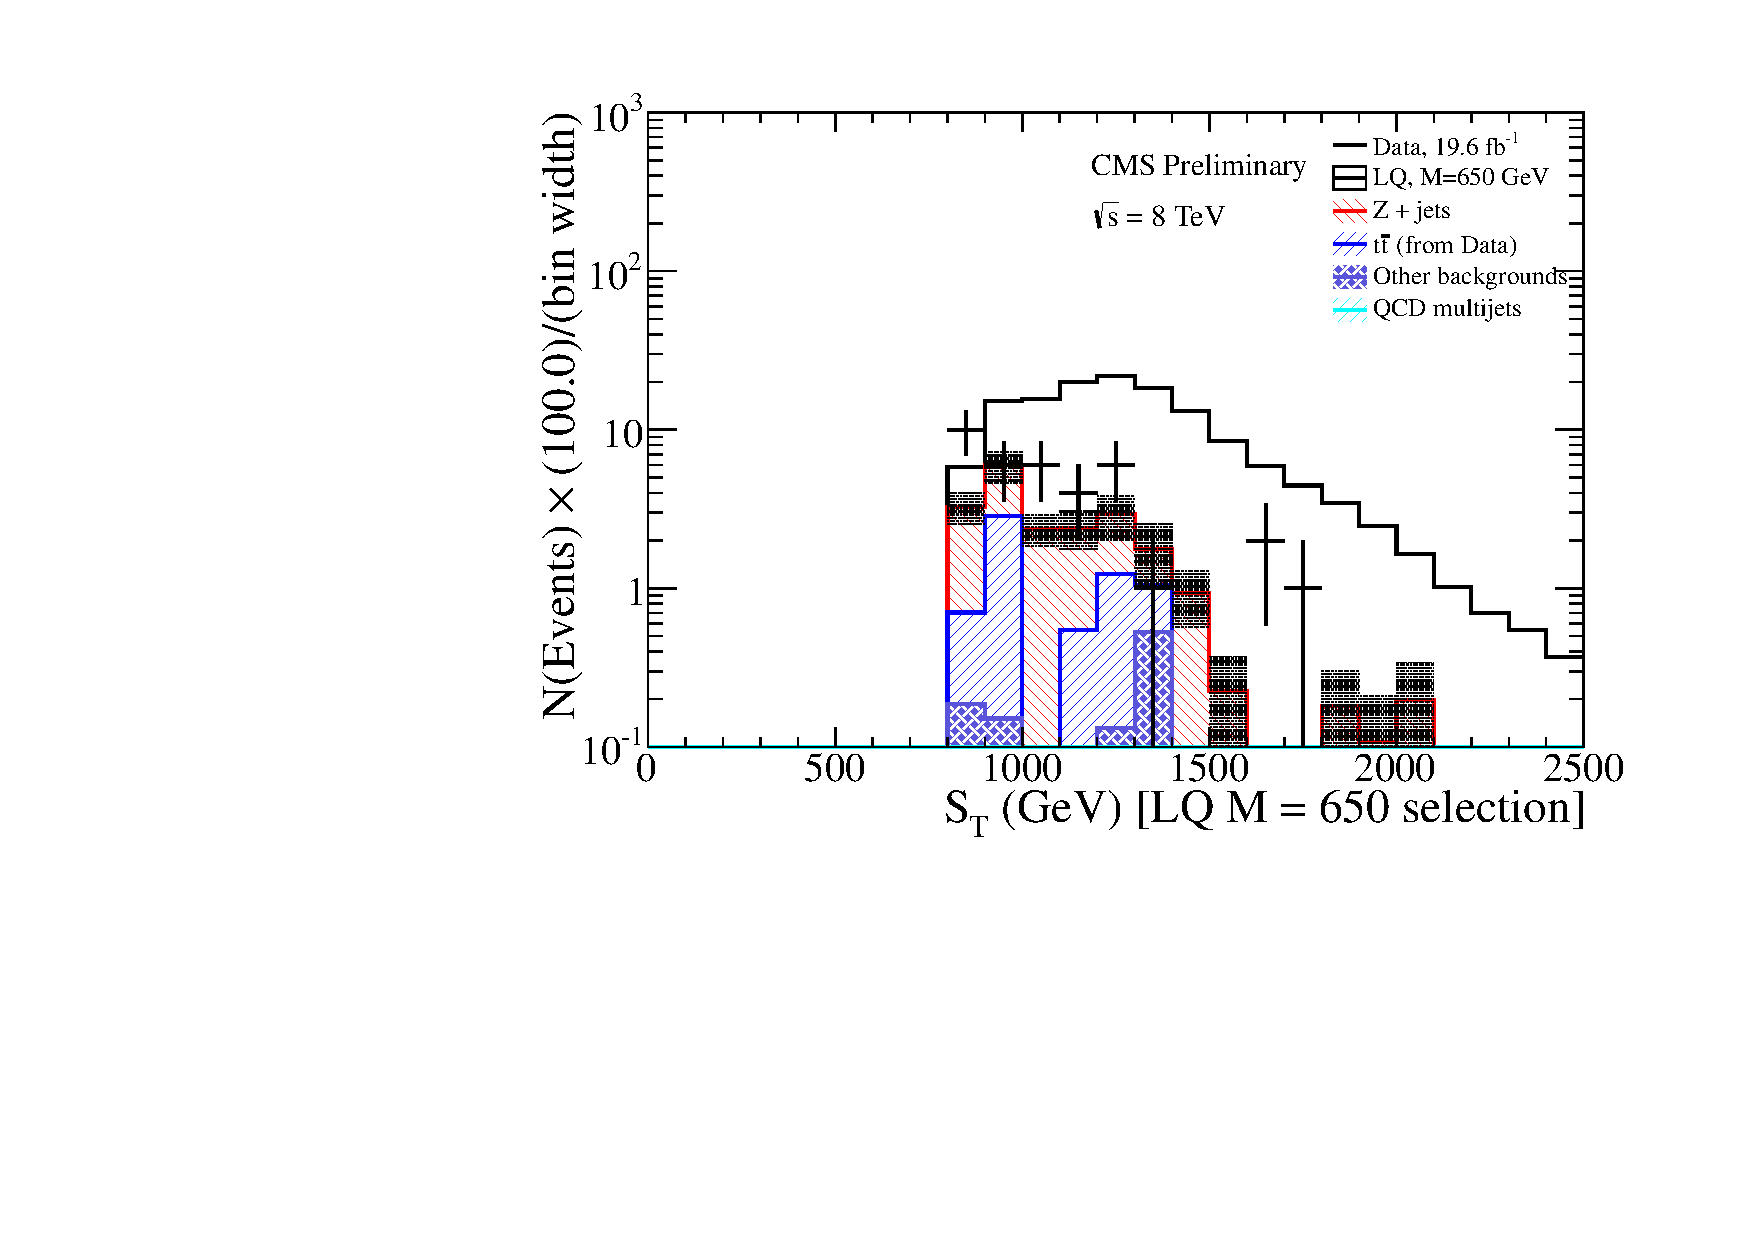
\includegraphics[width=\textwidth]{fig/ee/finalSelection/sT_eejj_LQ650_eejj.pdf}
\end{column}
\begin{column}{0.6\textwidth}
%% MEJ
\label{sec-2-4-2-2}

\centering
\mejmin
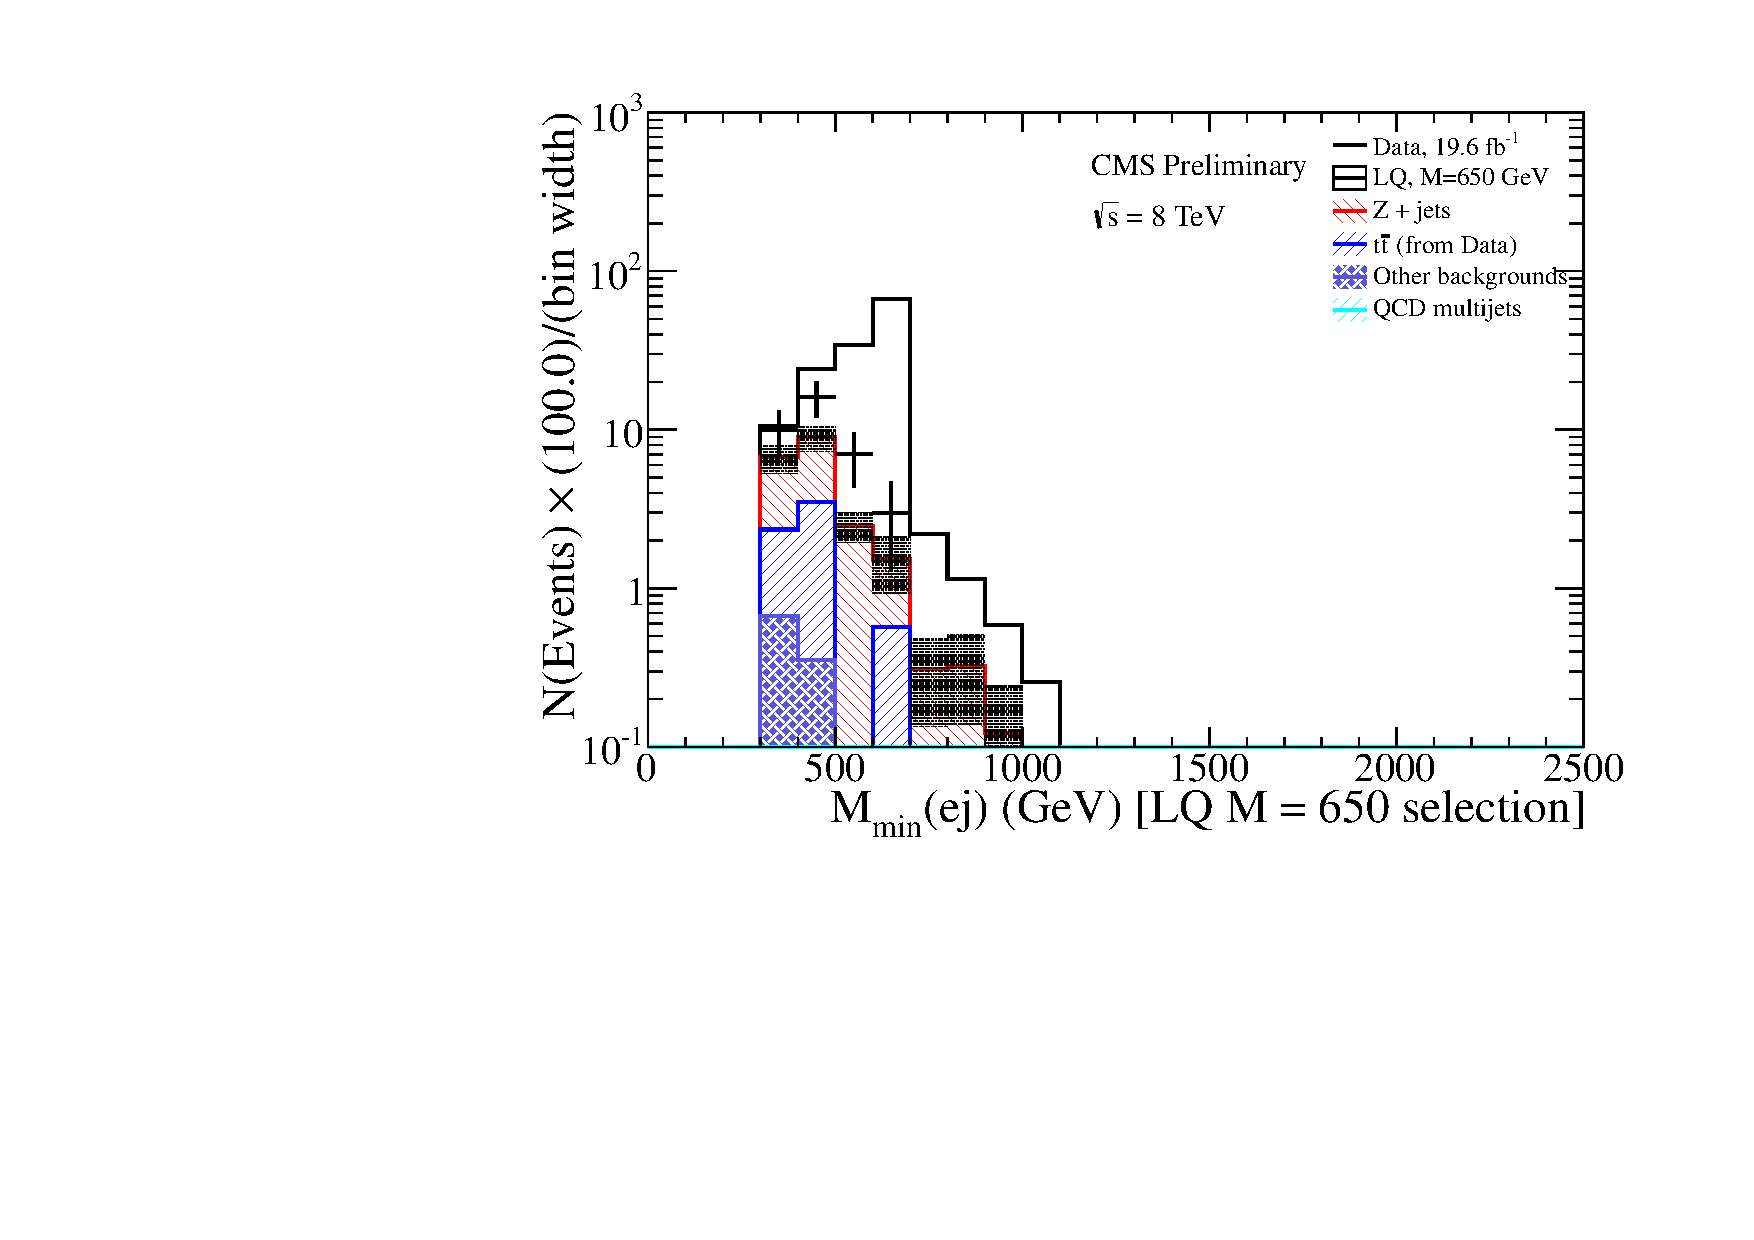
\includegraphics[width=\textwidth]{fig/ee/finalSelection/Mej_selected_min_LQ650_eejj.pdf}
\end{column}
\end{columns}
\end{frame}
\section{\enujj analysis}
\label{sec-3}
\subsection{\enujj preselection}
\label{sec-3-1}
\begin{frame}
\frametitle{\enujj preselection definition}
\label{sec-3-1-1}
%% Text
\label{sec-3-1-1-1}

\begin{itemize}
\item Exactly one electron: $\pt > 45$ GeV and  $|\eta| < 2.2$
\item $\met > 55$ GeV
\item At least two jets
\item $\pt(j_1) > 125$ GeV and $|\eta| < 2.4$
\item $\pt(j_2) > 45$  GeV and $|\eta| < 2.4$
\item $|\Delta\phi(e, \met)| > 0.5$
\item $|\Delta\phi(j_1, \met)| > 0.5$
\item $\mt > 50$ GeV
\item $\ST = \pt(e_1) + \met + \pt(j_1) + \pt(j_2) > 300$ GeV
\item Muon veto
\item Same trigger as \eejj analysis
\end{itemize}
\end{frame}
\begin{frame}
\frametitle{\enujj preselection: \ST and \mej}
\label{sec-3-1-2}
\begin{columns}
\begin{column}{0.6\textwidth}
%% ST
\label{sec-3-1-2-1}

\centering
$\ST$
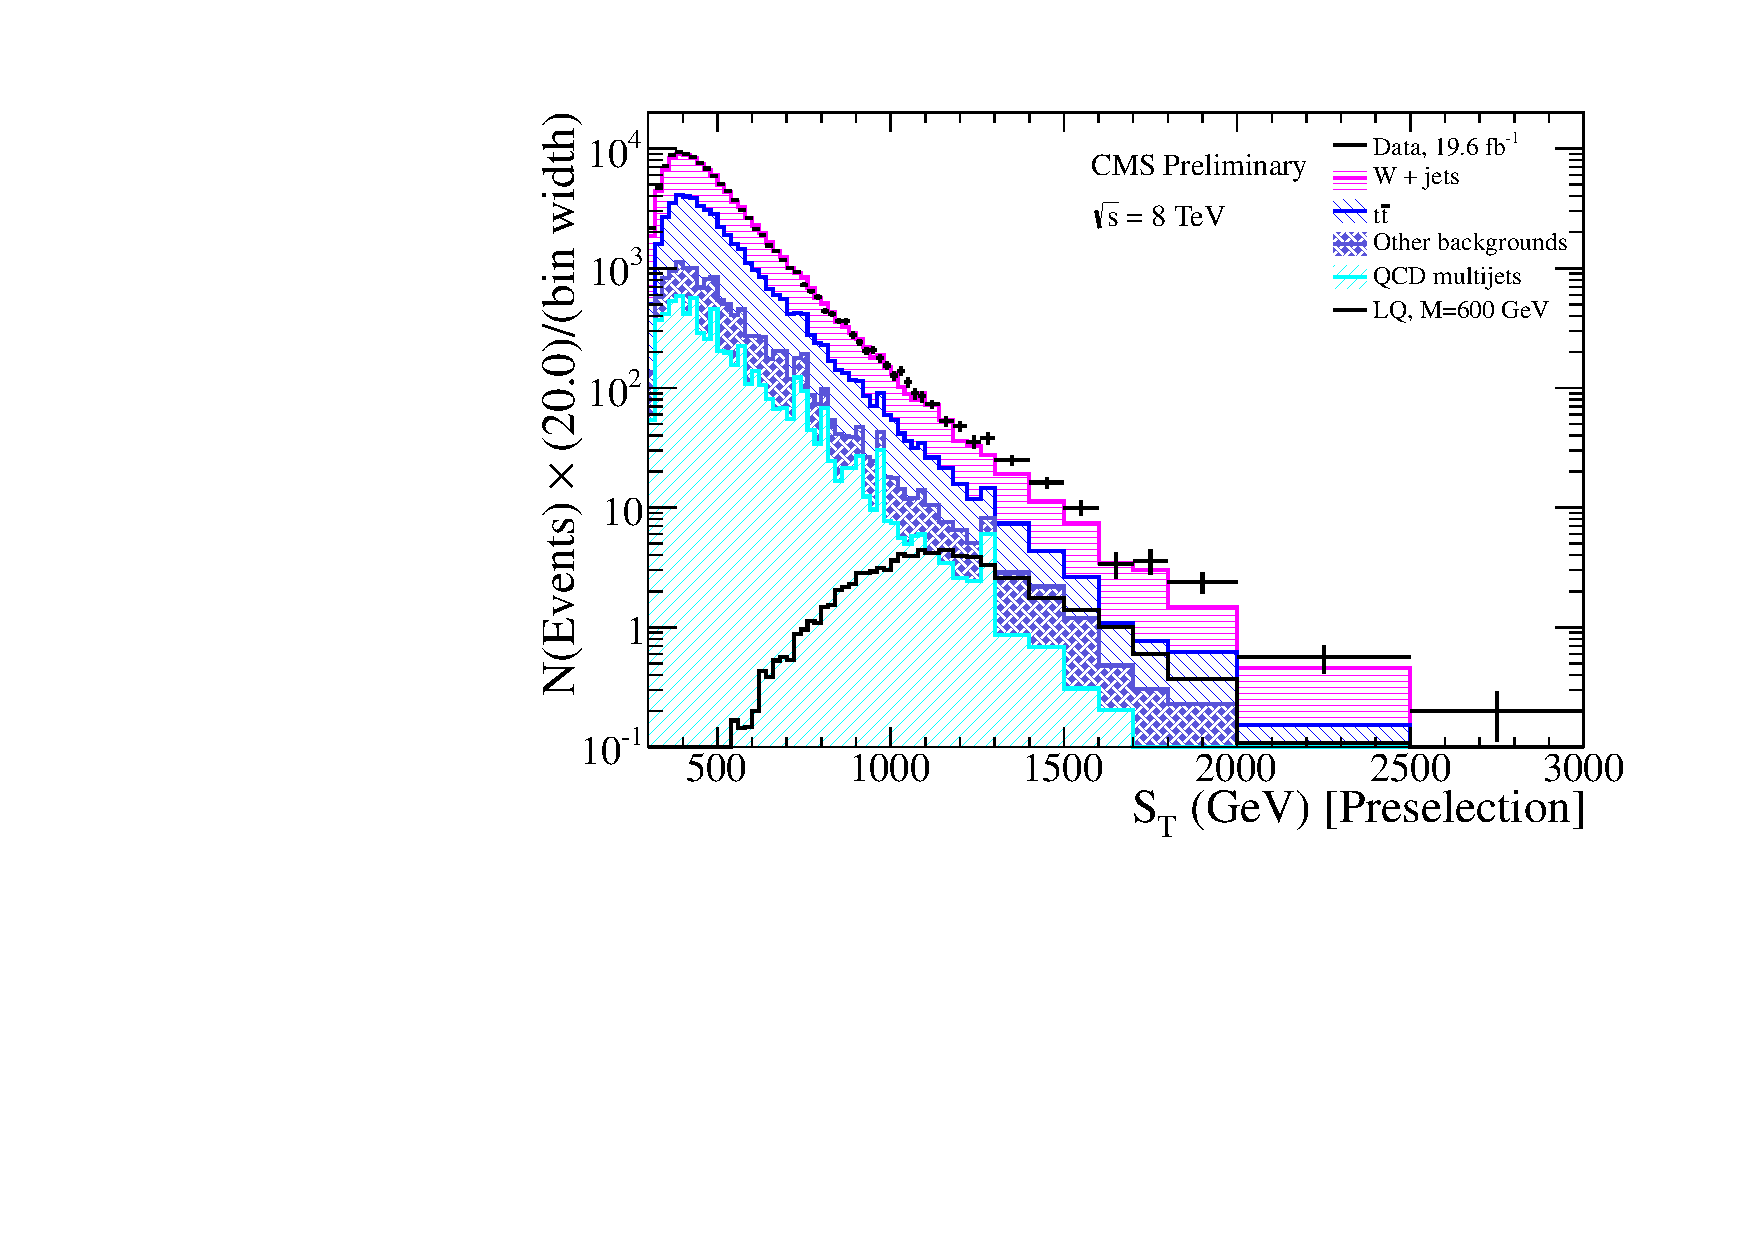
\includegraphics[width=\textwidth]{fig/enu/preselection_noRatio/sT_PAS_enujj.pdf}
\end{column}
\begin{column}{0.6\textwidth}
%% MEJ
\label{sec-3-1-2-2}

\centering
\mej
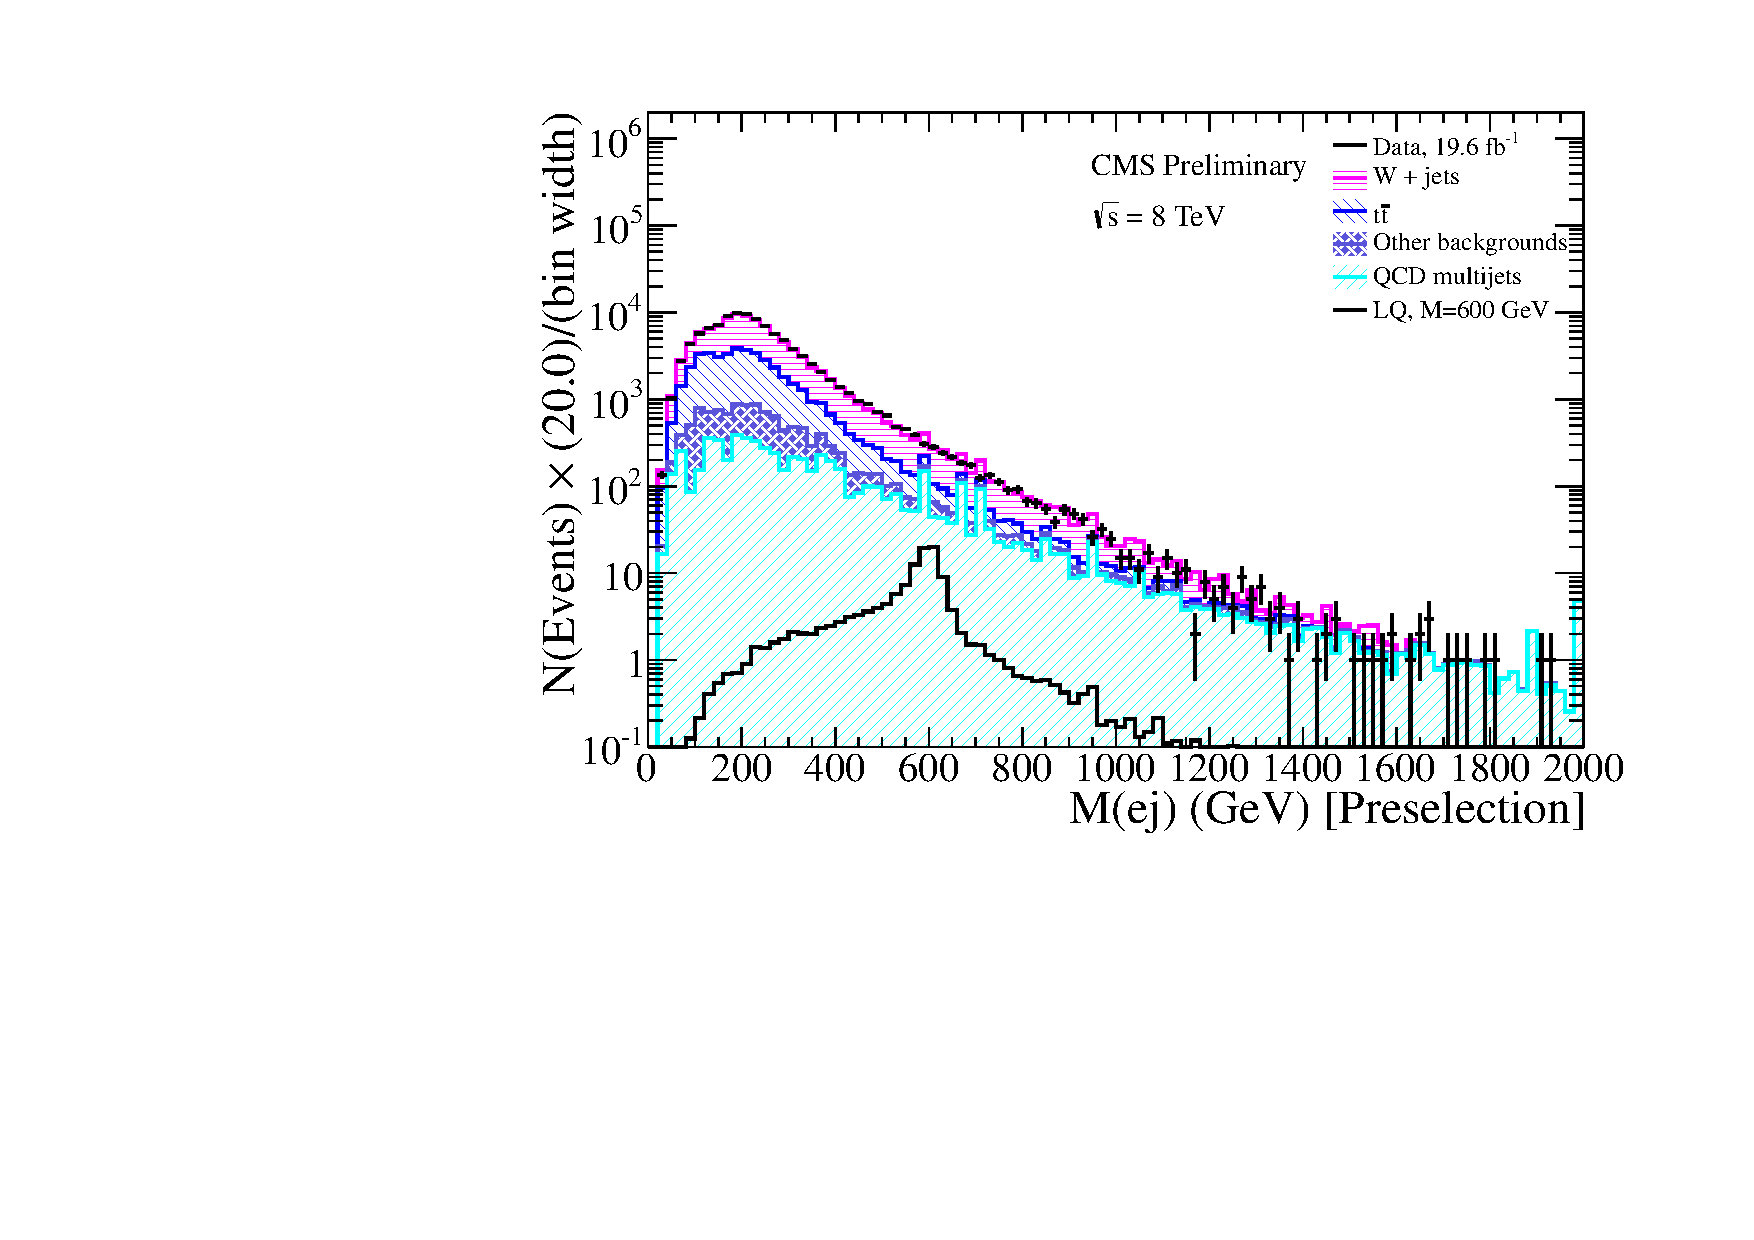
\includegraphics[width=\textwidth]{fig/enu/preselection_noRatio/Mej_PAS_enujj.pdf}
\end{column}
\end{columns}
\end{frame}
\subsection{\enujj backgrounds}
\label{sec-3-2}
\begin{frame}
\frametitle{\enujj backgrounds}
\label{sec-3-2-1}
\begin{block}{Backgrounds include:}
\label{sec-3-2-1-1}
\begin{itemize}

\item \ttbar: shape from MC, normalization from data \\ (dominant background)
\label{sec-3-2-1-1-1}%

\item \wjets: shape from MC, normalization from data
\label{sec-3-2-1-1-2}%

\item QCD multijets: shape and normalization from data \\ (same as \eejj)
\label{sec-3-2-1-1-3}%

\item Other backgrounds: shape and normalization from MC
\label{sec-3-2-1-1-4}%
\end{itemize} % ends low level
\end{block}
\end{frame}
\subsection{\enujj optimization}
\label{sec-3-3}
\begin{frame}
\frametitle{\enujj final selection optimization table}
\label{sec-3-3-1}
%% Text
\label{sec-3-3-1-1}

\begin{itemize}
\item Optimize \ST, \mej, \mt, and \met after \eejj preselection
\begin{itemize}
\item $e$-$j$ and $\met$-$j$ pairs are chosen to minimize the difference between the transverse mass of each pair
\item \mej is the mass of the $e$-$j$ pair
\item \met is optimized to reduce QCD background
\end{itemize}
\item Optimization figure of merit is $S/\sqrt{S+B}$
\item Results:
\end{itemize}
%% Table
\label{sec-3-3-1-2}

\resizebox{\textwidth}{!}{
\begin{tabular}{l|c|c|c|c|c|c|c|c|c|c|c|c|c|c|}
\cline{2-15} 
& \multicolumn{14}{c|}{LQ Mass (evjj)} \\ 
\cline{2-15} 
& 300 & 350 & 400 & 450 & 500 & 550 & 600 & 650 & 700 & 750 & 800 & 850 & 900 & $\ge 950$ \\
\hline 
\hline 
\multicolumn{1}{|c|}{\ST [GeV]}  & 495 & 570 & 645 & 720 & 800 & 880 & 960 & 1040 & 1120 & 1205 & 1290 & 1375 & 1460 & 1545 \\
\multicolumn{1}{|c|}{\met [GeV]}  & 90 & 95 & 100 & 110 & 115 & 125 & 135 & 145 & 155 & 170 & 180 & 195 & 210 & 220 \\
\multicolumn{1}{|c|}{\mej [GeV]}  & 195 & 250 & 300 & 355 & 405 & 455 & 505 & 555 & 600 & 645 & 695 & 740 & 780 & 825 \\
\multicolumn{1}{|c|}{\mt [GeV]}  & 125 & 150 & 175 & 200 & 220 & 240 & 255 & 270 & 280 & 290 & 295 & 300 & 300 & 300 \\
\hline 
\end{tabular}            
}%
\end{frame}
\subsection{\enujj final selection}
\label{sec-3-4}
\begin{frame}
\frametitle{\enujj final selection table}
\label{sec-3-4-1}
%% Table
\label{sec-3-4-1-1}

\resizebox{\textwidth}{!}{
\begin{tikzpicture}
\node (table) {
      \begin{tabular}{| l | c | c | c | c | c | c | c | c |} 
        \hline 
        $M_{LQ}$ & LQ Signal & W+Jets & $t\bar{t}$ & QCD & Other & Data &  Total Background & Significance \\ 
        \hline 
        \hline 
        Presel & - &  $ 58284.8 \pm 197.0 $ & $ 32196.7 \pm 69.8 $ & $ 5950.5 \pm 20.1 $ & $ 6590.8 \pm 231.6 $ &105164 & $ 103022.8 \pm 312.6 $ & NA \\ 
        \hline 
        300 &  $ 4765.5\pm 51.1 $ &  $ 822.1 \pm 22.4 $ & $ 1191.3 \pm 12.0 $ & $ 117.9 \pm 1.5 $ & $ 210.5 \pm 7.7 $ & 2455 &  $ 2341.90 \pm 26.58 $ $ \pm $ $ 329.79 $ (syst) & 0.3 \\ 
        350 &  $ 2168.4\pm 21.6 $ &  $ 275.9 \pm 14.5 $ & $ 441.4 \pm 7.2 $ & $ 59.11 \pm 0.97 $ & $ 102.1 \pm 5.4 $ & 908 &  $ 878.55 \pm 17.08 $ $ \pm $ $ 122.13 $ (syst) & 0.2 \\ 
        400 &  $ 971.1\pm 9.6 $ &  $ 110.4 \pm 7.8 $ & $ 184.2 \pm 4.7 $ & $ 32.88 \pm 0.69 $ & $ 51.5 \pm 3.8 $ & 413 &  $ 378.98 \pm 9.91 $ $ \pm $ $ 51.38 $ (syst) & 0.5 \\ 
        450 &  $ 469.7\pm 4.6 $ &  $ 53.1 \pm 5.8 $ & $ 74.7 \pm 3.0 $ & $ 14.13 \pm 0.42 $ & $ 25.7 \pm 2.7 $ & 192 &  $ 167.64 \pm 7.06 $ $ \pm $ $ 21.33 $ (syst) & 0.8 \\ 
        500 &  $ 232.7\pm 2.3 $ &  $ 20.5 \pm 3.3 $ & $ 34.4 \pm 2.0 $ & $ 7.76 \pm 0.30 $ & $ 15.3 \pm 2.1 $ & 83 &  $ 77.99 \pm 4.41 $ $ \pm $ $ 9.77 $ (syst) & 0.0 \\ 
        550 &  $ 121.4\pm 1.2 $ &  $ 8.6 \pm 1.8 $ & $ 14.9 \pm 1.4 $ & $ 3.89 \pm 0.21 $ & $ 7.8 \pm 1.6 $ & 44 &  $ 35.24 \pm 2.76 $ $ \pm $ $ 4.31 $ (syst) & 1.0 \\ 
        600 &  $ 66.37\pm 0.66 $ &  $ 2.3 \pm 1.0 $ & $ 7.08 \pm 0.93 $ & $ 2.29 \pm 0.17 $ & $ 4.6 \pm 1.2 $ & 28 &  $ 16.27 \pm 1.84 $ $ \pm $ $ 2.03 $ (syst) & 2.1 \\ 
        650 &  $ 37.22\pm 0.37 $ &  $ 0.41 \pm 0.29 $ & $ 3.82 \pm 0.70 $ & $ 1.18 \pm 0.12 $ & $ 2.13 \pm 0.92 $ & 18 &  $ 7.54 \pm 1.20 $ $ \pm $ $ 1.07 $ (syst) & 2.6 \\ 
        700 &  $ 21.74\pm 0.21 $ &  $ 0.41 \pm 0.29 $ & $ 2.61 \pm 0.60 $ & $ 0.85 \pm 0.10 $ & $ 0.58 \pm 0.24 $ & 6 &  $ 4.45 \pm 0.71 $ $ \pm $ $ 0.74 $ (syst) & 0.0 \\ 
        750 &  $ 12.90\pm 0.13 $ &  $ 0.00_{-0.00}^{+0.94}$ &  $ 1.75 \pm 0.47 $ & $ 0.514 \pm 0.091 $ & $ 0.27 \pm 0.15 $ & 4 &  $ 2.535_{-0.504}^{+1.062}$ $ \pm $ $ 0.49 $ (syst)  & 0.0 \\ 
        800 &  $ 7.610\pm 0.075 $ &  $ 0.00_{-0.00}^{+0.94}$ &  $ 1.10 \pm 0.37 $ & $ 0.317 \pm 0.067 $ & $ 0.27 \pm 0.15 $ & 3 &  $ 1.696_{-0.404}^{+1.019}$ $ \pm $ $ 0.31 $ (syst)  & 0.0 \\ 
        850 &  $ 4.713\pm 0.046 $ &  $ 0.00_{-0.00}^{+0.94}$ &  $ 0.90 \pm 0.34 $ & $ 0.117 \pm 0.029 $ & $ 0.140 \pm 0.087 $ & 2 &  $ 1.153_{-0.353}^{+0.999}$ $ \pm $ $ 0.24 $ (syst)  & 0.0 \\ 
        900 &  $ 2.929\pm 0.028 $ &  $ 0.00_{-0.00}^{+0.94}$ &  $ 0.37 \pm 0.21 $ & $ 0.076 \pm 0.024 $ & $ 0.084 \pm 0.069 $ & 1 &  $ 0.530_{-0.226}^{+0.962}$ $ \pm $ $ 0.10 $ (syst)  & 0.0 \\ 
        950 &  $ 1.839\pm 0.018 $ &  $ 0.00_{-0.00}^{+0.94}$ &  $ 0.37 \pm 0.21 $ & $ 0.069 \pm 0.023 $ & $ 0.084 \pm 0.069 $ & 1 &  $ 0.524_{-0.226}^{+0.962}$ $ \pm $ $ 0.10 $ (syst)  & 0.0 \\ 
        1000 &  $ 1.306\pm 0.012 $ &  $ 0.00_{-0.00}^{+0.94}$ &  $ 0.37 \pm 0.21 $ & $ 0.069 \pm 0.023 $ & $ 0.084 \pm 0.069 $ & 1 &  $ 0.524_{-0.226}^{+0.962}$ $ \pm $ $ 0.10 $ (syst)  & 0.0 \\ 
        1050 &  $ 0.9022\pm 0.0076 $ &  $ 0.00_{-0.00}^{+0.94}$ &  $ 0.37 \pm 0.21 $ & $ 0.069 \pm 0.023 $ & $ 0.084 \pm 0.069 $ & 1 &  $ 0.524_{-0.226}^{+0.962}$ $ \pm $ $ 0.10 $ (syst)  & 0.0 \\ 
        1100 &  $ 0.6225\pm 0.0050 $ &  $ 0.00_{-0.00}^{+0.94}$ &  $ 0.37 \pm 0.21 $ & $ 0.069 \pm 0.023 $ & $ 0.084 \pm 0.069 $ & 1 &  $ 0.524_{-0.226}^{+0.962}$ $ \pm $ $ 0.10 $ (syst)  & 0.0 \\ 
        1150 &  $ 0.4308\pm 0.0032 $ &  $ 0.00_{-0.00}^{+0.94}$ &  $ 0.37 \pm 0.21 $ & $ 0.069 \pm 0.023 $ & $ 0.084 \pm 0.069 $ & 1 &  $ 0.524_{-0.226}^{+0.962}$ $ \pm $ $ 0.10 $ (syst)  & 0.0 \\ 
        1200 &  $ 0.2971\pm 0.0022 $ &  $ 0.00_{-0.00}^{+0.94}$ &  $ 0.37 \pm 0.21 $ & $ 0.069 \pm 0.023 $ & $ 0.084 \pm 0.069 $ & 1 &  $ 0.524_{-0.226}^{+0.962}$ $ \pm $ $ 0.10 $ (syst)  & 0.0 \\ 
        \hline 
      \end{tabular}

};
\draw [red,ultra thick,rounded corners]
($(table.south west) !.52! (table.north west)$)
rectangle 
($(table.south east) !.57! (table.north east)$);    
\draw [red,ultra thick,rounded corners]
($(table.north east) !.385! (table.north west)$)
rectangle 
($(table.south east) !0.! (table.north west)$);    
\end{tikzpicture}
}%
%% Text
\label{sec-3-4-1-2}

\begin{itemize}
\item Broad excess of data w.r.t. total background (as in \eejj)
\item Most significant for $M_{\text{LQ}} = 650$ GeV selection (as in \eejj)
\end{itemize}
\end{frame}
\begin{frame}
\frametitle{\enujj final selection (650): \ST and \mej ($\beta = 0.5$)}
\label{sec-3-4-2}
\begin{columns}
\begin{column}{0.6\textwidth}
%% ST
\label{sec-3-4-2-1}

\centering
\ST
\includegraphics[width=\textwidth]{fig/enu/finalSelection/sT_LQ650_enujj.pdf}
\end{column}
\begin{column}{0.6\textwidth}
%% MEJ
\label{sec-3-4-2-2}

\centering
\mej
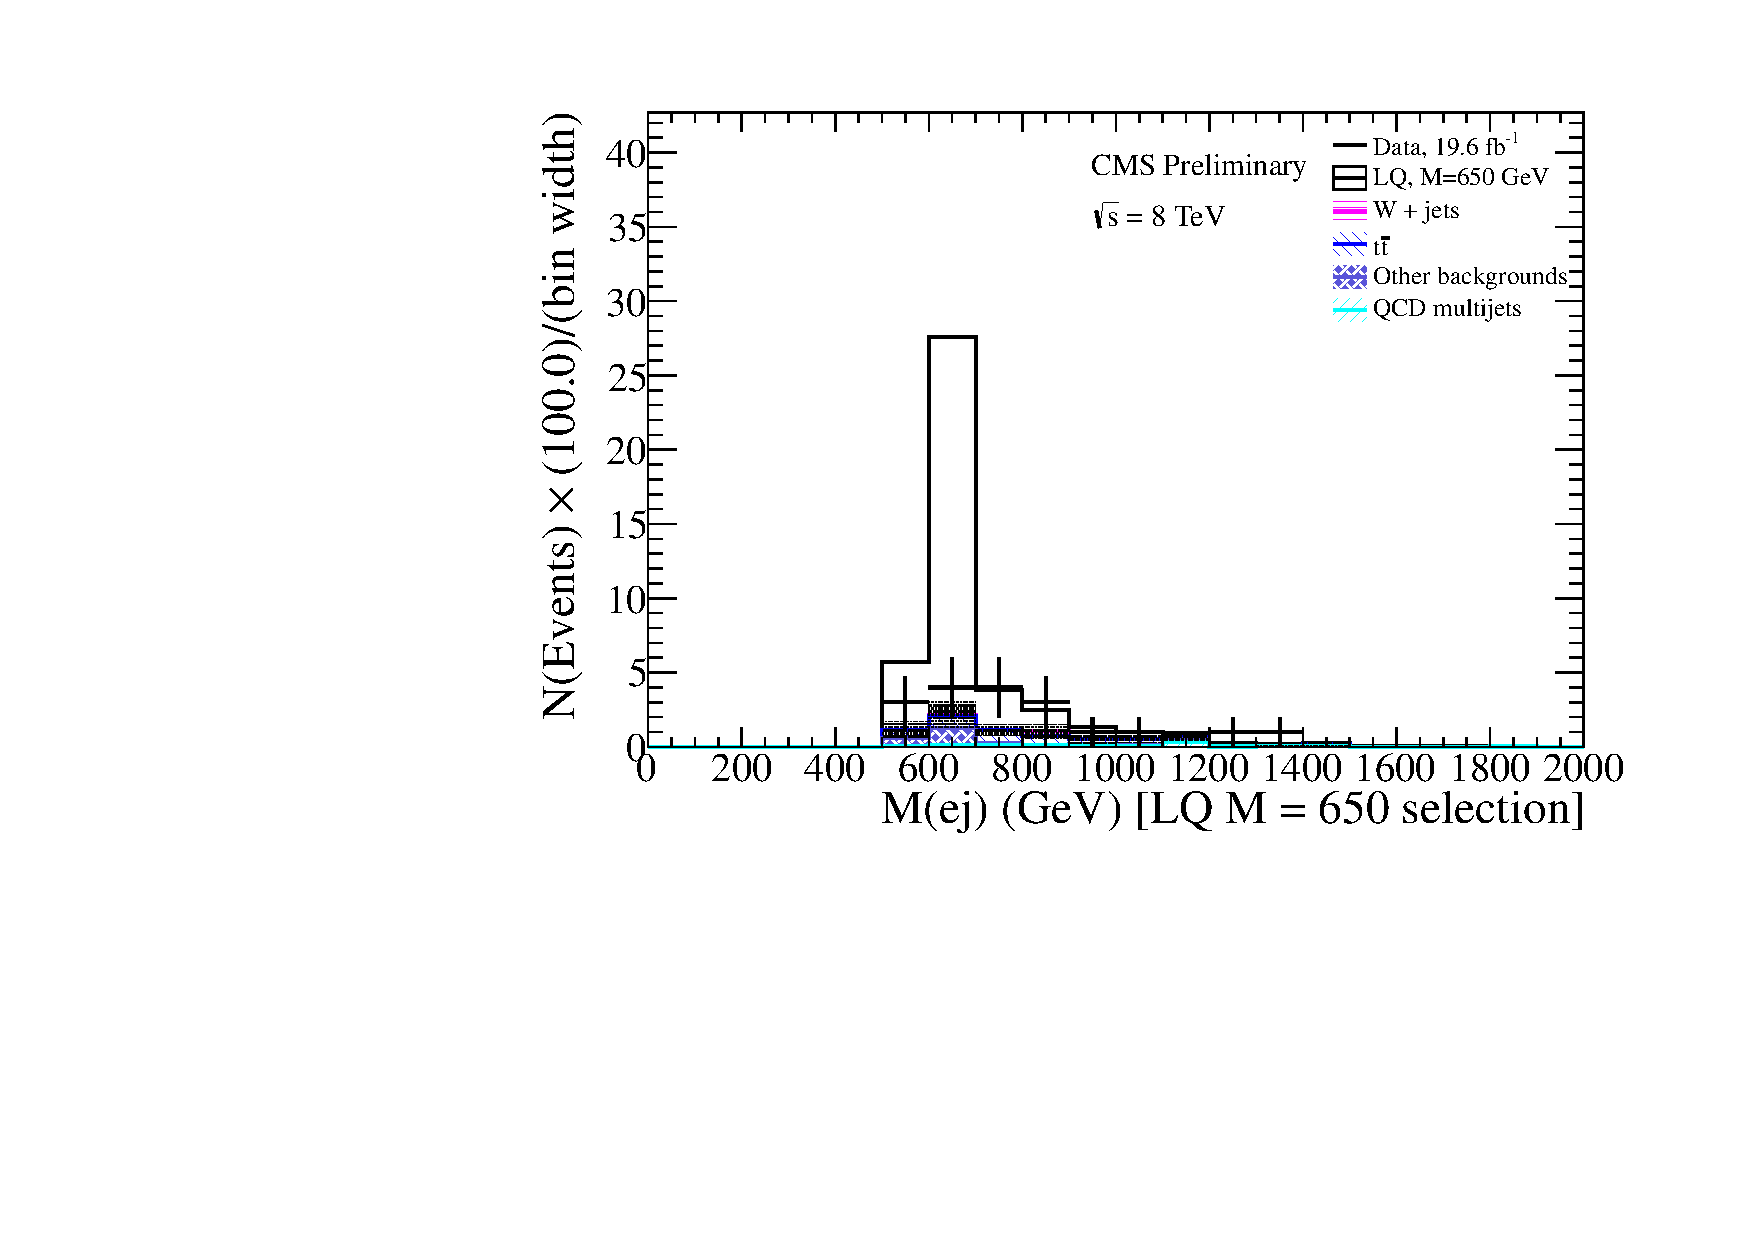
\includegraphics[width=\textwidth]{fig/enu/finalSelection/Mej_LQ650_enujj.pdf}
\end{column}
\end{columns}
\end{frame}
\section{Systematics}
\label{sec-4}
\subsection{Systematic uncertainties: overview}
\label{sec-4-1}
\begin{frame}
\frametitle{Systematic uncertainties}
\label{sec-4-1-1}
\begin{columns} % Columns
\label{sec-4-1-1-1}
\begin{column}{0.55\textwidth}
%% Column 1
\label{sec-4-1-1-1-1}

\ChangeItemFont{\footnotesize}{\footnotesize}{\footnotesize}
\begin{itemize}
\item Background MC shape (varies):
\begin{itemize}
\item \wjets and \ttbar in \enujj
\item \zjets in \eejj
\end{itemize}
\item PDF (varies)
\item Jet energy scale (varies)
\item Jet energy resolution: \\
eta-dependent, 5-30\%
\item Electron energy scale: \\
0.4\% barrel, 4.1\% endcap
\item Electron energy resolution: \\
0.6\% barrel, 1.5\% endcap
\end{itemize}
\end{column}
\begin{column}{0.55\textwidth}
%% Column 2
\label{sec-4-1-1-1-2}

\ChangeItemFont{\footnotesize}{\footnotesize}{\footnotesize}
\begin{itemize}
\item Background MC normalization:
\begin{itemize}
\item \wjets (2\%) in \enujj
\item \ttbar (2\%) in \enujj
\item \zjets (1\%) in \eejj
\end{itemize}
\item QCD normalization: \\
60\% (30\%) in \eejj (\enujj)
\item \ttbar normalization in \eejj: 2\%
\item Electron reco/ID/Iso effi: \\
4\% (2\%) in \eejj (\enujj) signal
\item Pileup
\item Luminosity: 2.6\%
\item MC statistics: \alert{Dominates}
\end{itemize}
\end{column}
\end{columns}
\end{frame}
\section{Results}
\label{sec-5}
\subsection{Standalone limits}
\label{sec-5-1}
\begin{frame}
\frametitle{Results: standalone limits}
\label{sec-5-1-1}
\begin{columns} % Plots
\label{sec-5-1-1-1}
\begin{column}{0.5\textwidth}
%% eejj limit
\label{sec-5-1-1-1-1}

\centering
$\beta = 1.0$
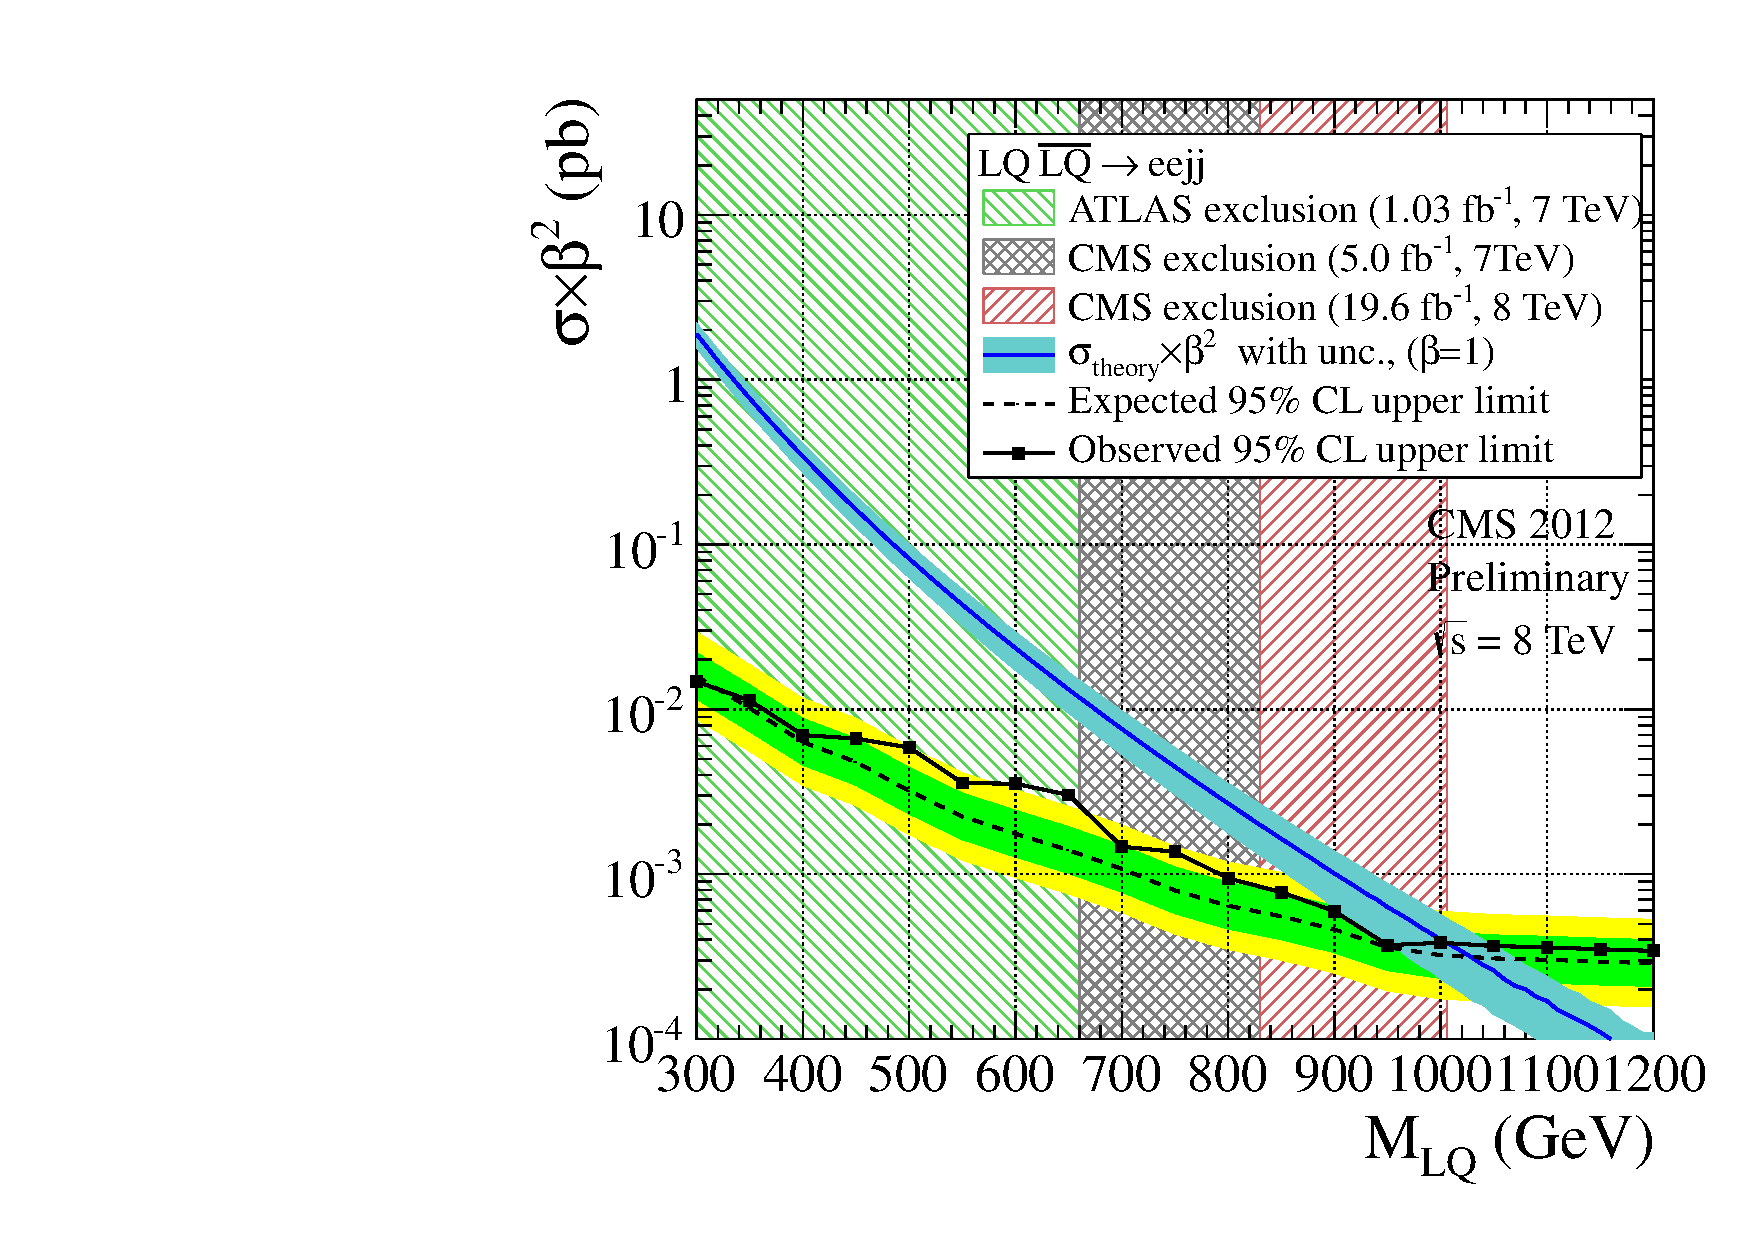
\includegraphics[width=0.875\textwidth]{fig/limits/BR_Sigma_EE.pdf}
\end{column}
\begin{column}{0.5\textwidth}
%% enujj limit
\label{sec-5-1-1-1-2}

\centering
$\beta = 0.5$
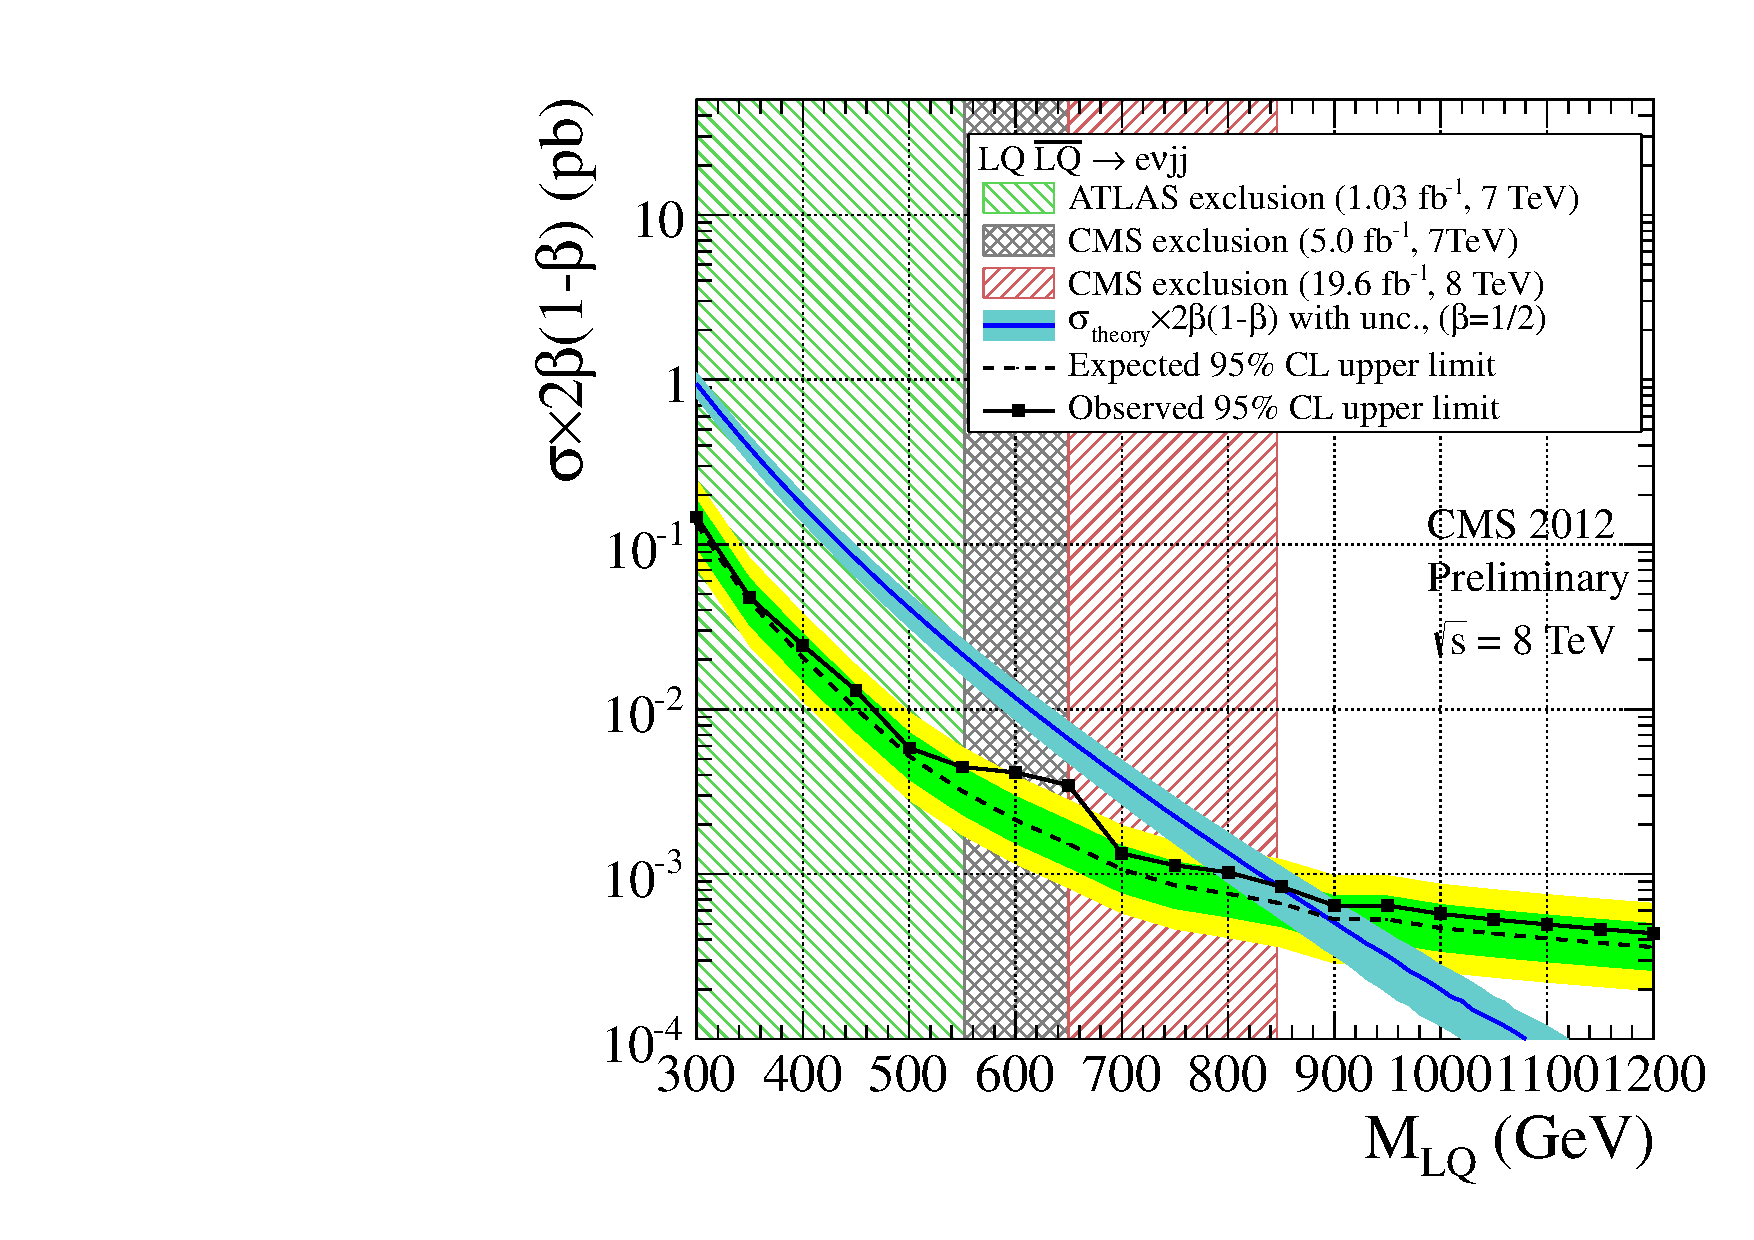
\includegraphics[width=0.875\textwidth]{fig/limits/BR_Sigma_ENu.pdf}
\end{column}
\end{columns}
%% Notes
\label{sec-5-1-1-2}

\begin{itemize}
\item Expected limits: $M_{LQ} < \eejjExpectedLimit$ $(\enujjExpectedLimit)$ GeV for \eejj (\enujj)
\item Observed limits: $M_{LQ} < \eejjObservedLimit$ $(\enujjObservedLimit)$ GeV for \eejj (\enujj)
\end{itemize}
\end{frame}
\subsection{Combined limits}
\label{sec-5-2}
\begin{frame}
\frametitle{Results: combined limits}
\label{sec-5-2-1}
\begin{columns} % Columns
\label{sec-5-2-1-1}
\begin{column}{0.5\textwidth}
%% Text
\label{sec-5-2-1-1-1}

\begin{itemize}
\item Made with asymptotic CLs
\item \enujj excess has strongest effect on combined limit discrepancy
\item Limits at $\beta = 0.15$:
\begin{itemize}
\item Exp.: $M_{LQ} < \lowBetaExpectedLimit$ GeV
\item Obs.: $M_{LQ} < \lowBetaObservedLimit$ GeV
\end{itemize}
\end{itemize}
\end{column}
\begin{column}{0.5\textwidth}
%% Plot
\label{sec-5-2-1-1-2}

\centering
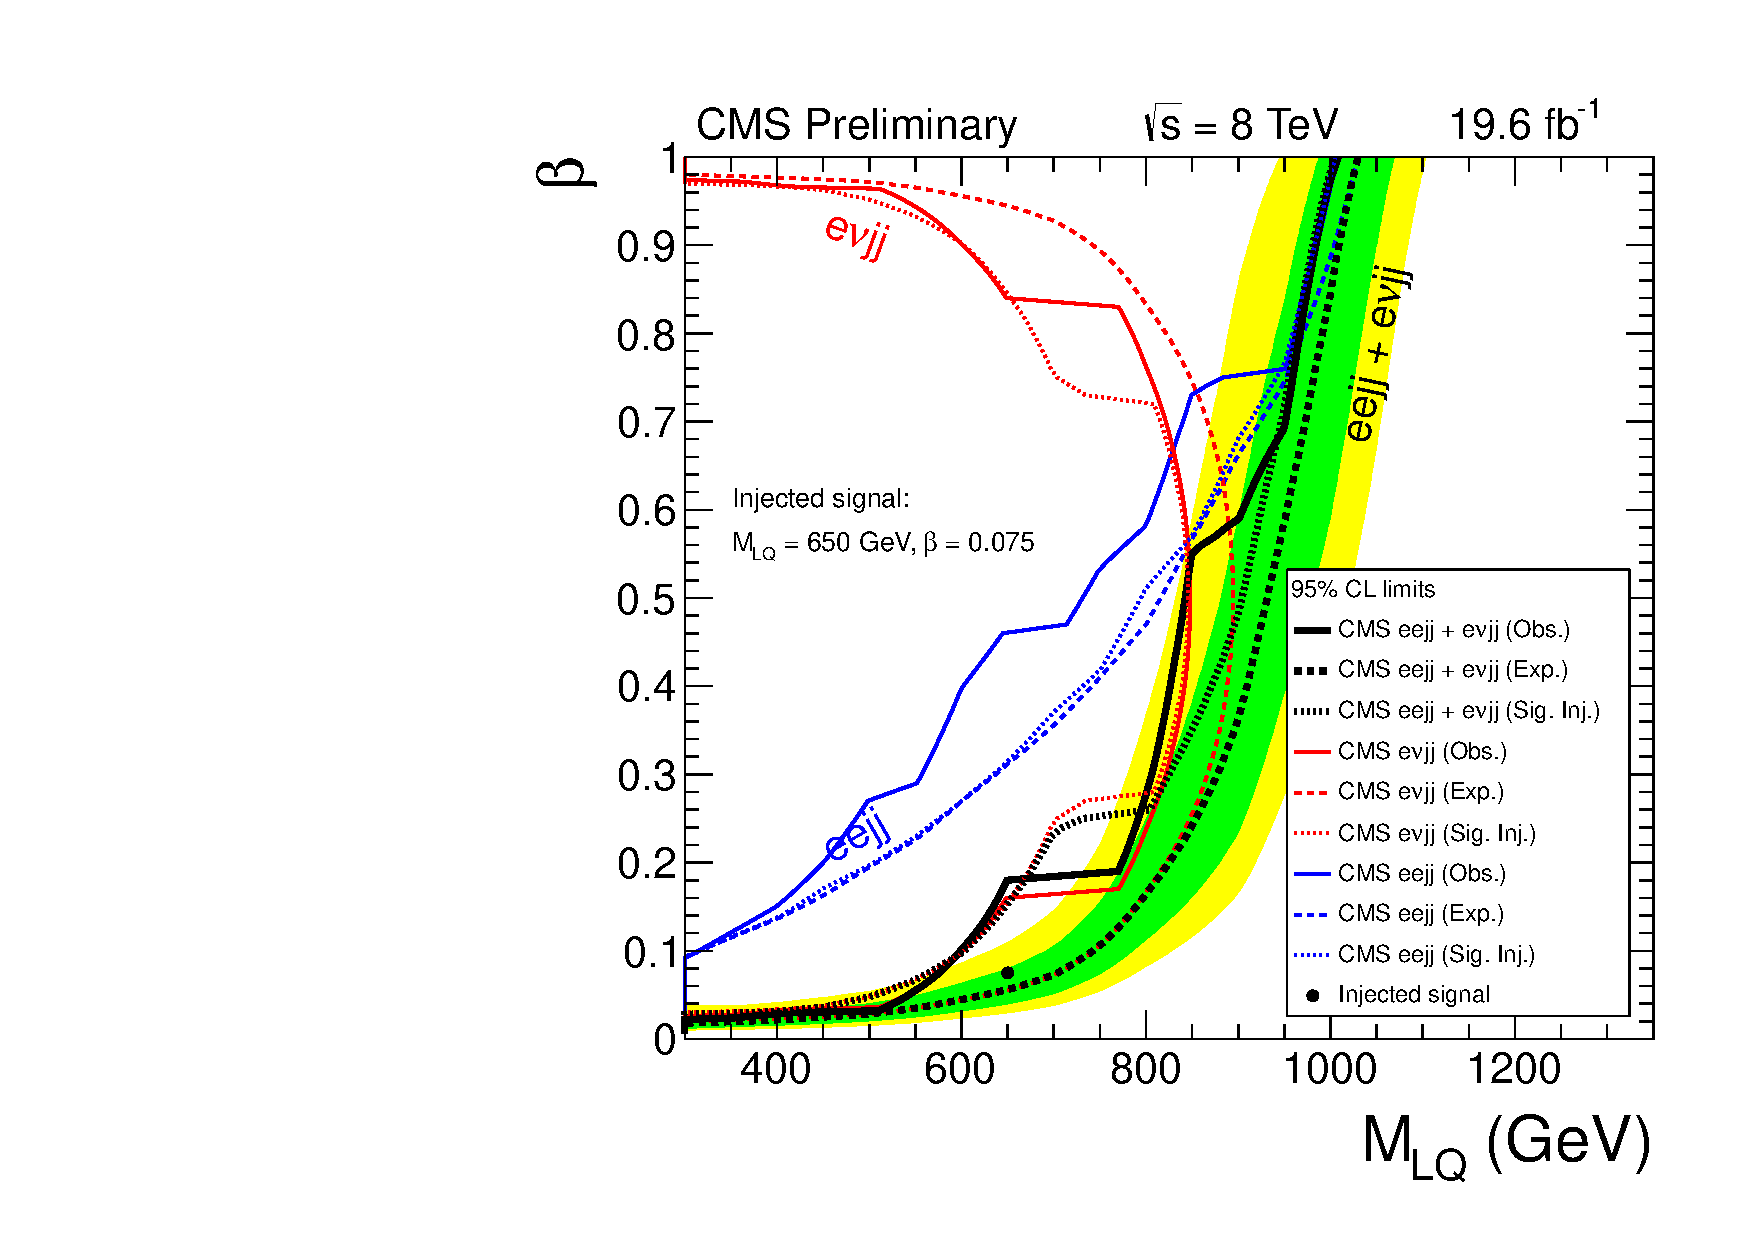
\includegraphics[width=\textwidth]{fig/limits/LQ1Combination_SignalInjection.pdf}
\end{column}
\end{columns}
\end{frame}
\section{Conclusion}
\label{sec-6}
\subsection{Conclusion}
\label{sec-6-1}
\begin{frame}
\frametitle{Conclusion}
\label{sec-6-1-1}
%% Text
\label{sec-6-1-1-1}

% \centering
% \resizebox*{!}{0.8\textheight}{\vbox{
\ChangeItemFont{\footnotesize}{\footnotesize}{\footnotesize}
\begin{itemize}
\item A search was carried out for first generation LQs in two channels:
\begin{itemize}
\item $\text{LQ}\overline{\text{LQ}}\rightarrow\eejj$  (optimized for $\beta = 1.0$)
\item $\text{LQ}\overline{\text{LQ}}\rightarrow\enujj$ (optimized for $\beta = 0.5$)
\end{itemize}
\item Combination of the channels sets world's best limits on leptoquarks at 95\% CL:
\begin{itemize}
\item Exp. limits: $M_{LQ} < \eejjExpectedLimit$ $(\enujjExpectedLimit)$ GeV for $\beta = 1.0$ (0.5)
\item Obs. limits: $M_{LQ} < \eejjObservedLimit$ $(\enujjObservedLimit)$ GeV for $\beta = 1.0$ (0.5)
\end{itemize}
\item With current data:
\begin{itemize}
\item We observe an excess of > $2\sigma$
\item We cannot exclude an LQ of mass 650 GeV with $\beta = 0.15$
\item Results have been extensively cross checked (see backup)
\end{itemize}
\end{itemize}
% }}
\end{frame}
\section{Backup}
\label{sec-7}
\subsection{Backup}
\label{sec-7-1}
\begin{frame}
\frametitle{Backup}
\label{sec-7-1-1}
\begin{itemize}

\item Read more:
\label{sec-7-1-1-1}%
\begin{itemize}

\item \href{http://indico.ific.uv.es/indico/materialDisplay.py?contribId=1023&sessionId=24&materialId=slides&confId=2025}{\alert{\underline{ICHEP talk}}}
\label{sec-7-1-1-1-1}%

\item \href{https://twiki.cern.ch/twiki/bin/view/CMSPublic/PhysicsResultsEXO12041}{\alert{\underline{Publicly available plots}}}
\label{sec-7-1-1-1-2}%

\item \href{http://inspirehep.net/record/1305762}{\alert{\underline{Publicly available analysis summary}}}
\label{sec-7-1-1-1-3}%
\end{itemize} % ends low level
\end{itemize} % ends low level
\end{frame}
\subsection{Beta = 0.15 N-1 plots}
\label{sec-7-2}
\begin{frame}
\frametitle{Results: $\beta = 0.075$, $M_{LQ} = 650$ (1/3)}
\label{sec-7-2-1}
\begin{columns}
\begin{column}{0.6\textwidth}
%% ST
\label{sec-7-2-1-1}

\centering
\ST
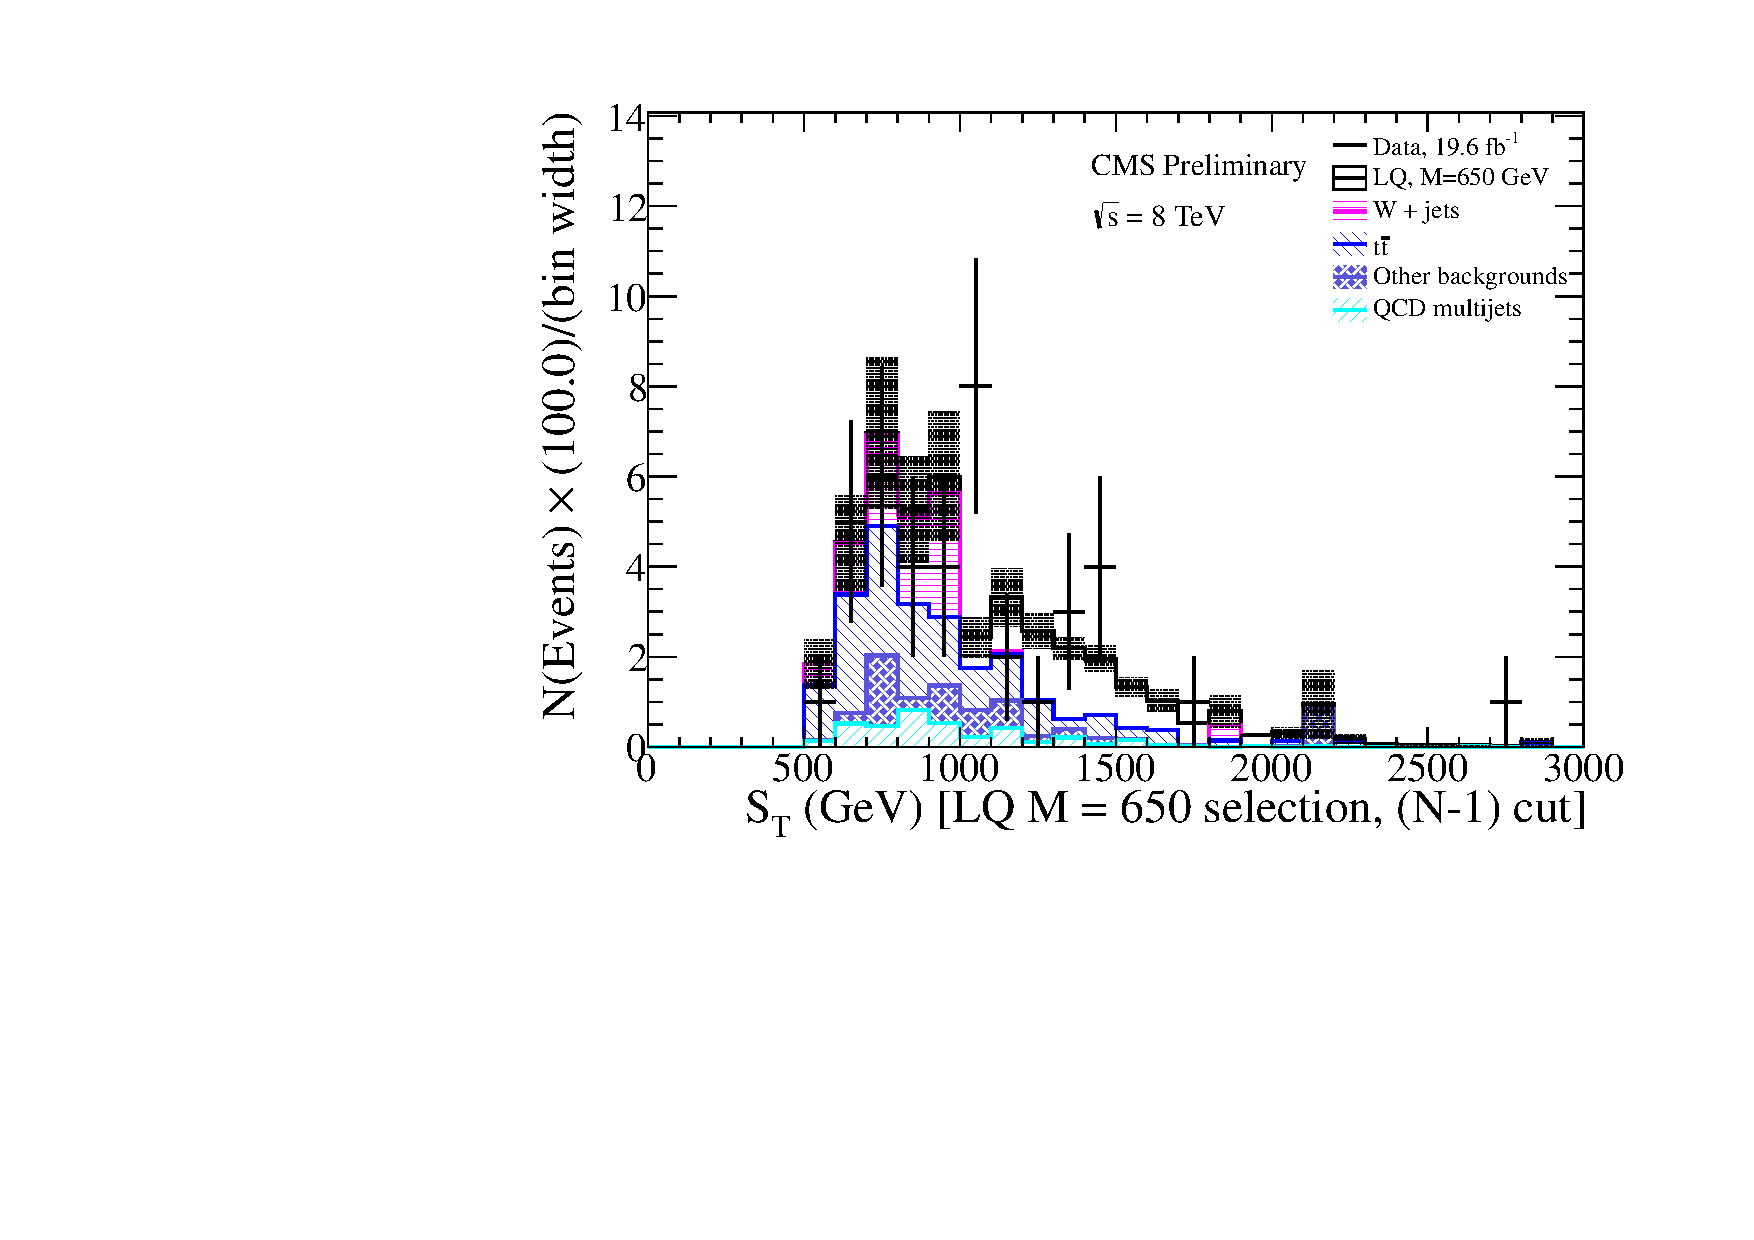
\includegraphics[width=\textwidth]{fig/enu/nMinus1/ST_mtAndMetAndMejLQ650_enujj.pdf}
\end{column}
\begin{column}{0.6\textwidth}
%% MEJ
\label{sec-7-2-1-2}

\centering
\mej
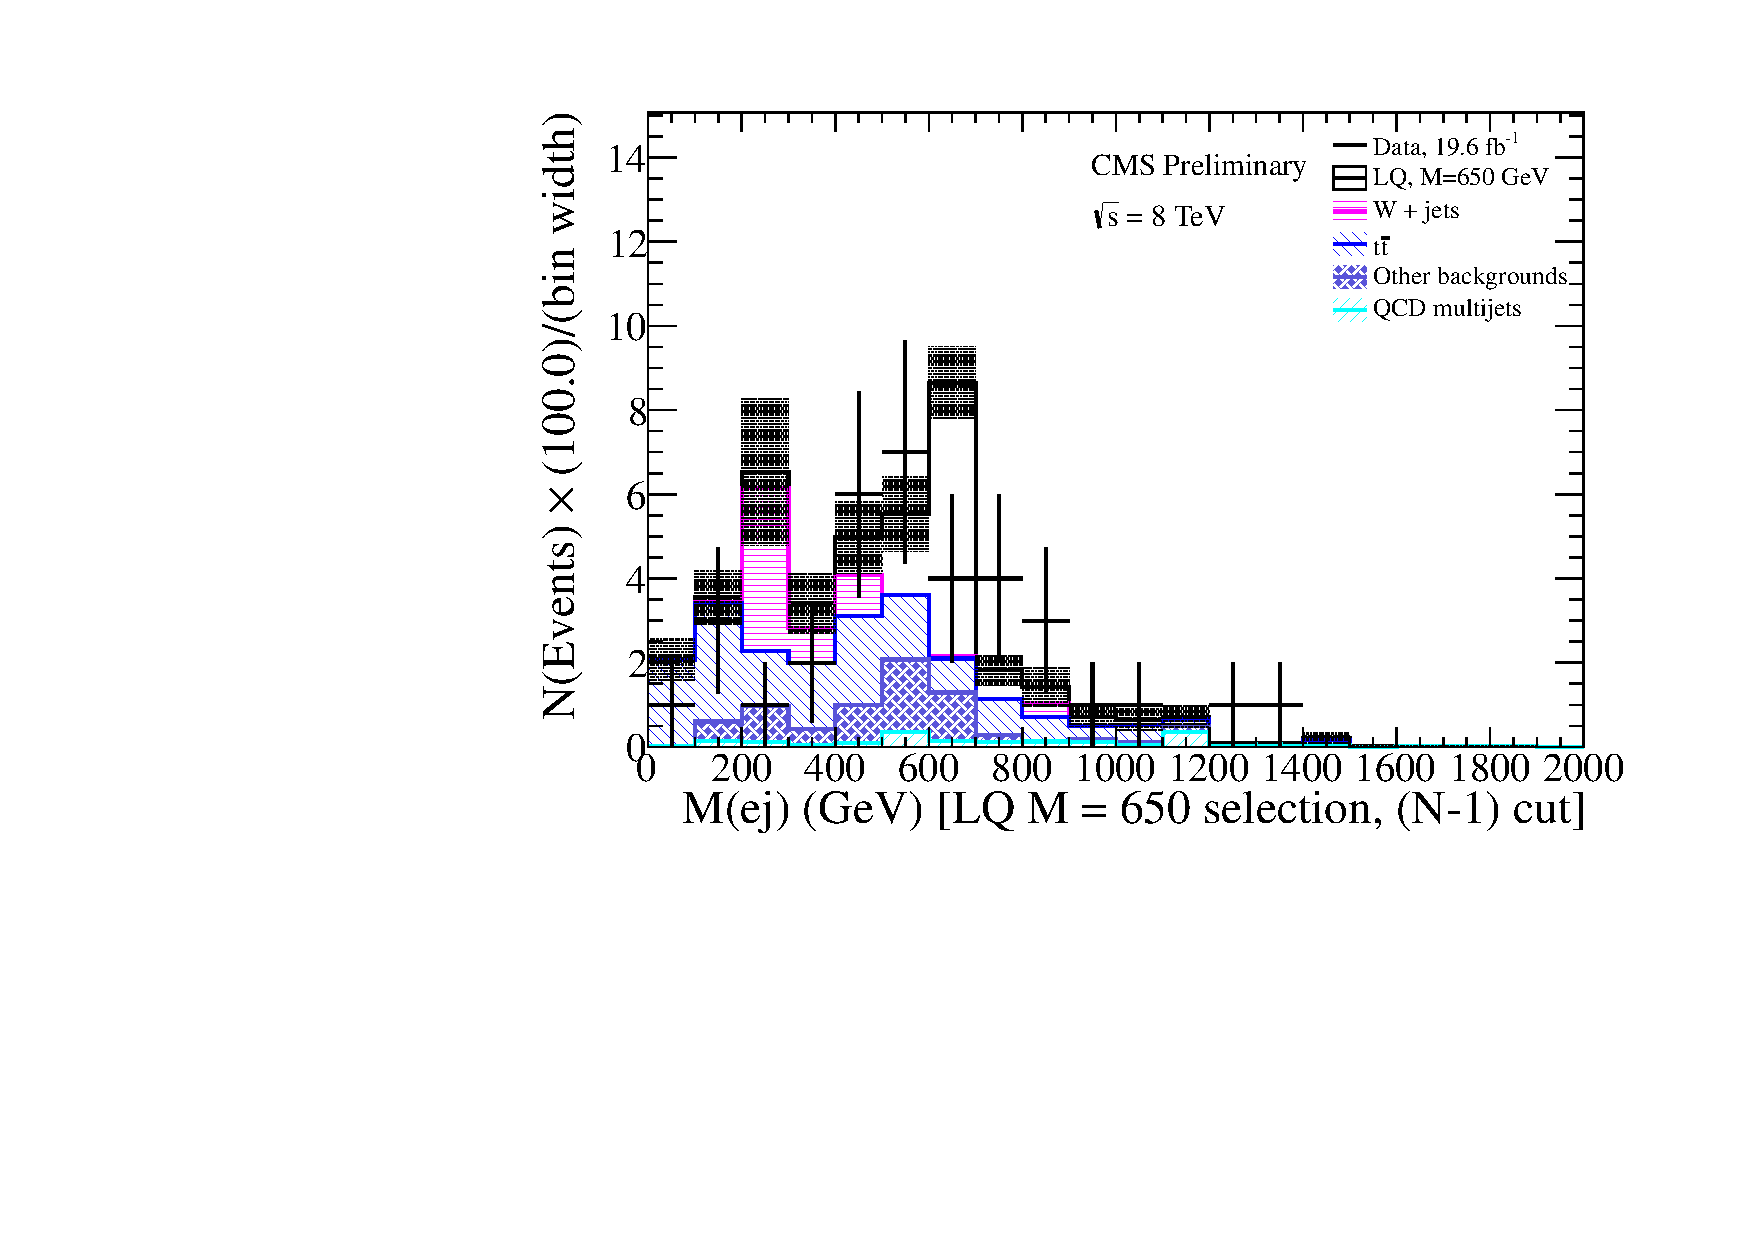
\includegraphics[width=\textwidth]{fig/enu/nMinus1/Mej_stAndMtAndMetLQ650_enujj.pdf}
\end{column}
\end{columns}
\end{frame}
\begin{frame}
\frametitle{Results: $\beta = 0.075$, $M_{LQ} = 650$ (2/3)}
\label{sec-7-2-2}
\begin{columns}
\begin{column}{0.6\textwidth}
%% MET
\label{sec-7-2-2-1}

\centering
\met
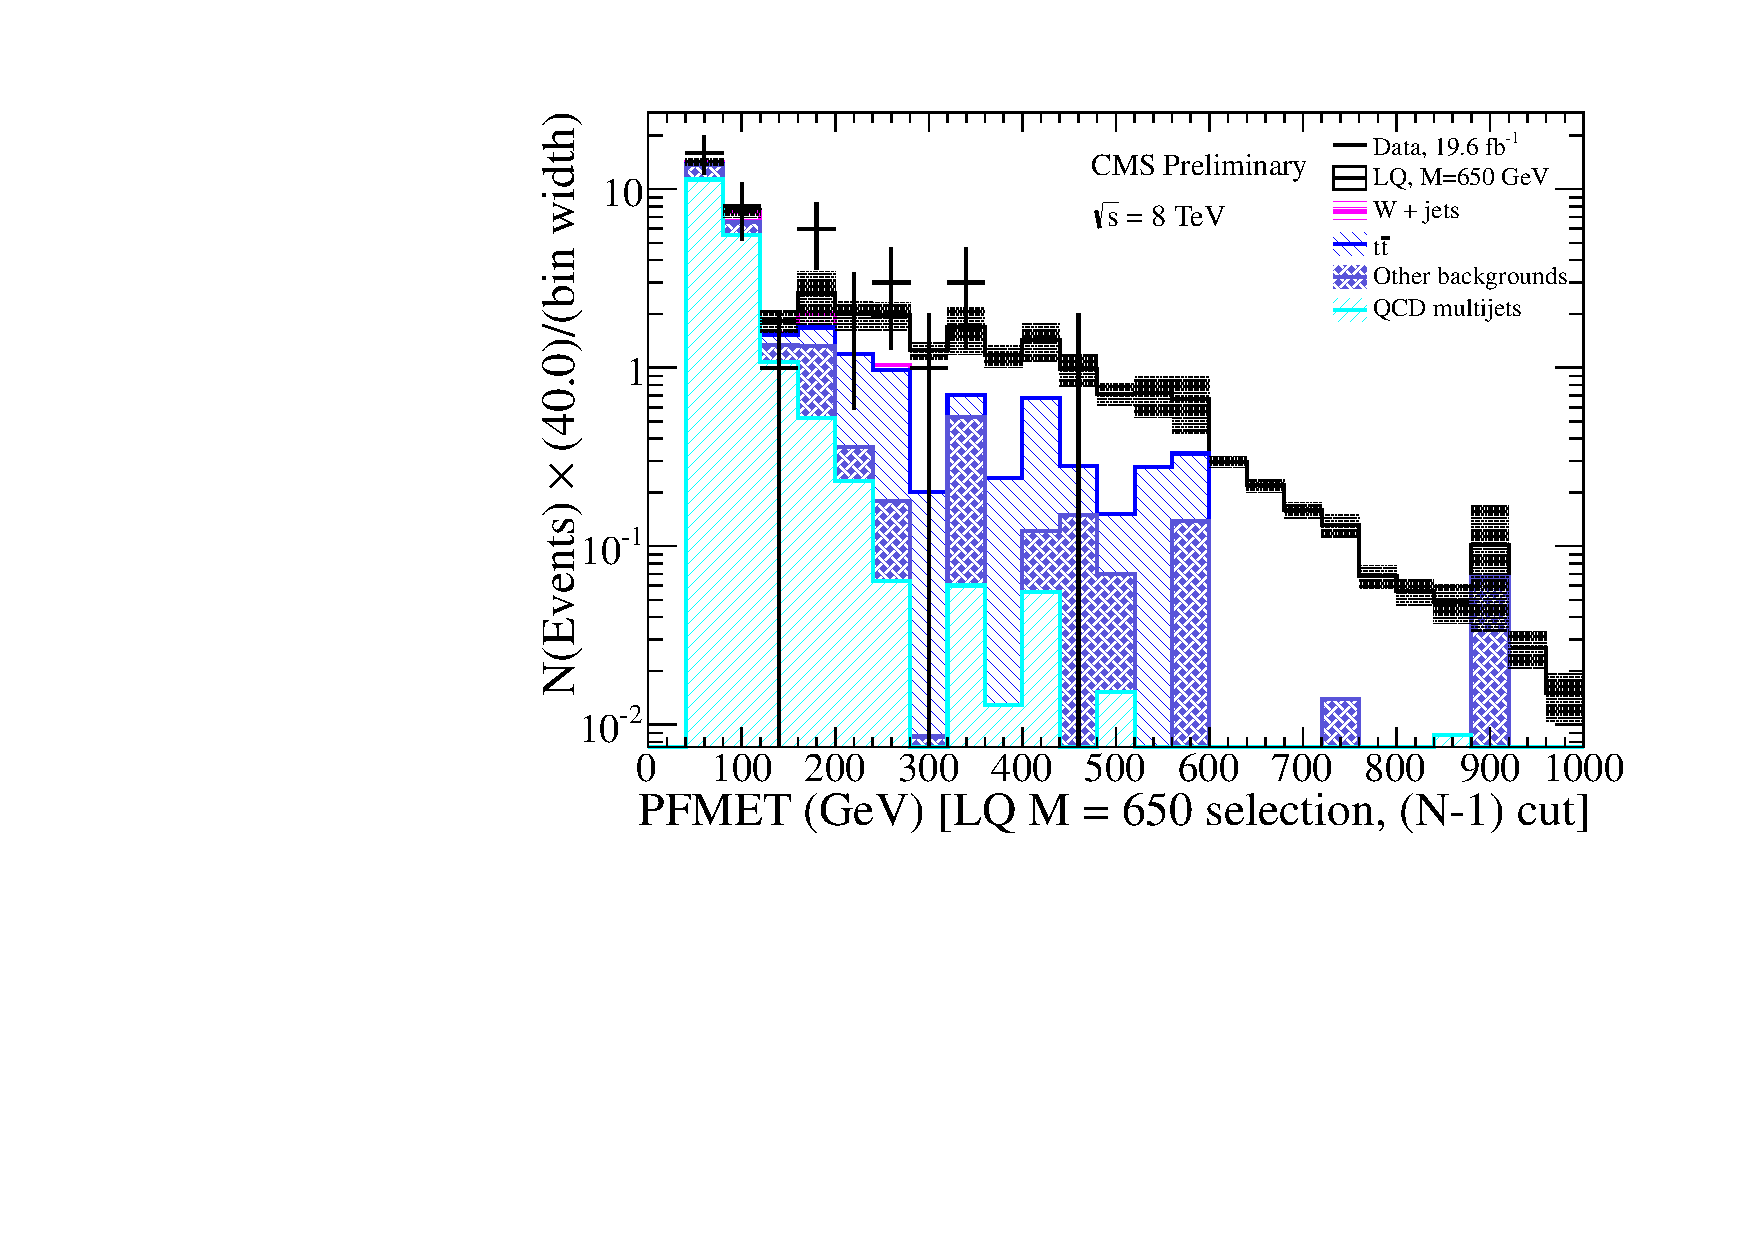
\includegraphics[width=\textwidth]{fig/enu/nMinus1/MET_stAndMtAndMejLQ650_enujj.pdf}
\end{column}
\begin{column}{0.6\textwidth}
%% MT
\label{sec-7-2-2-2}

\centering
\mt
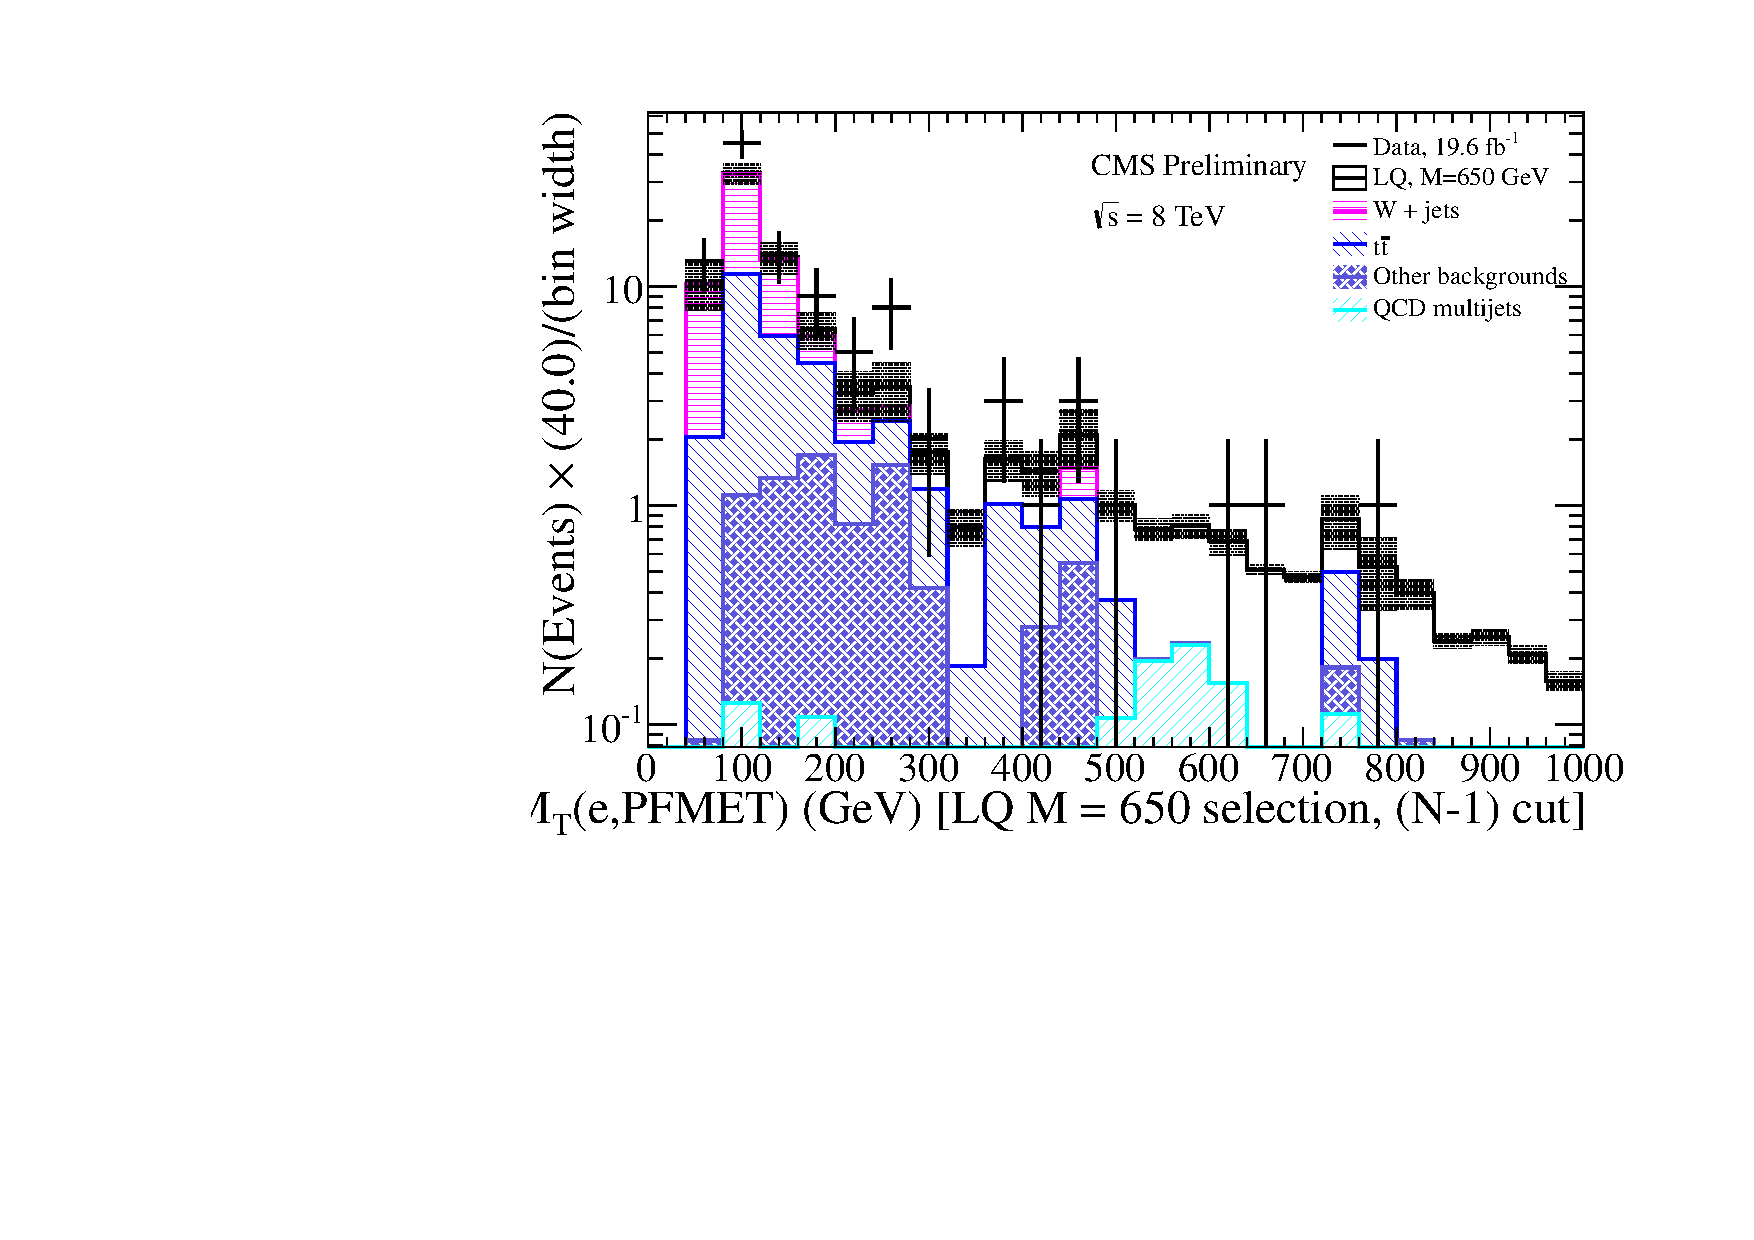
\includegraphics[width=\textwidth]{fig/enu/nMinus1/MTenu_stAndMetAndMejLQ650_enujj.pdf}
\end{column}
\end{columns}
\end{frame}
\begin{frame}
\frametitle{Results: $\beta = 0.075$, $M_{LQ} = 650$ (3/3)}
\label{sec-7-2-3}
\begin{columns}
\begin{column}{0.6\textwidth}
%% MT(j,nu)
\label{sec-7-2-3-1}

\centering
\mtjnu
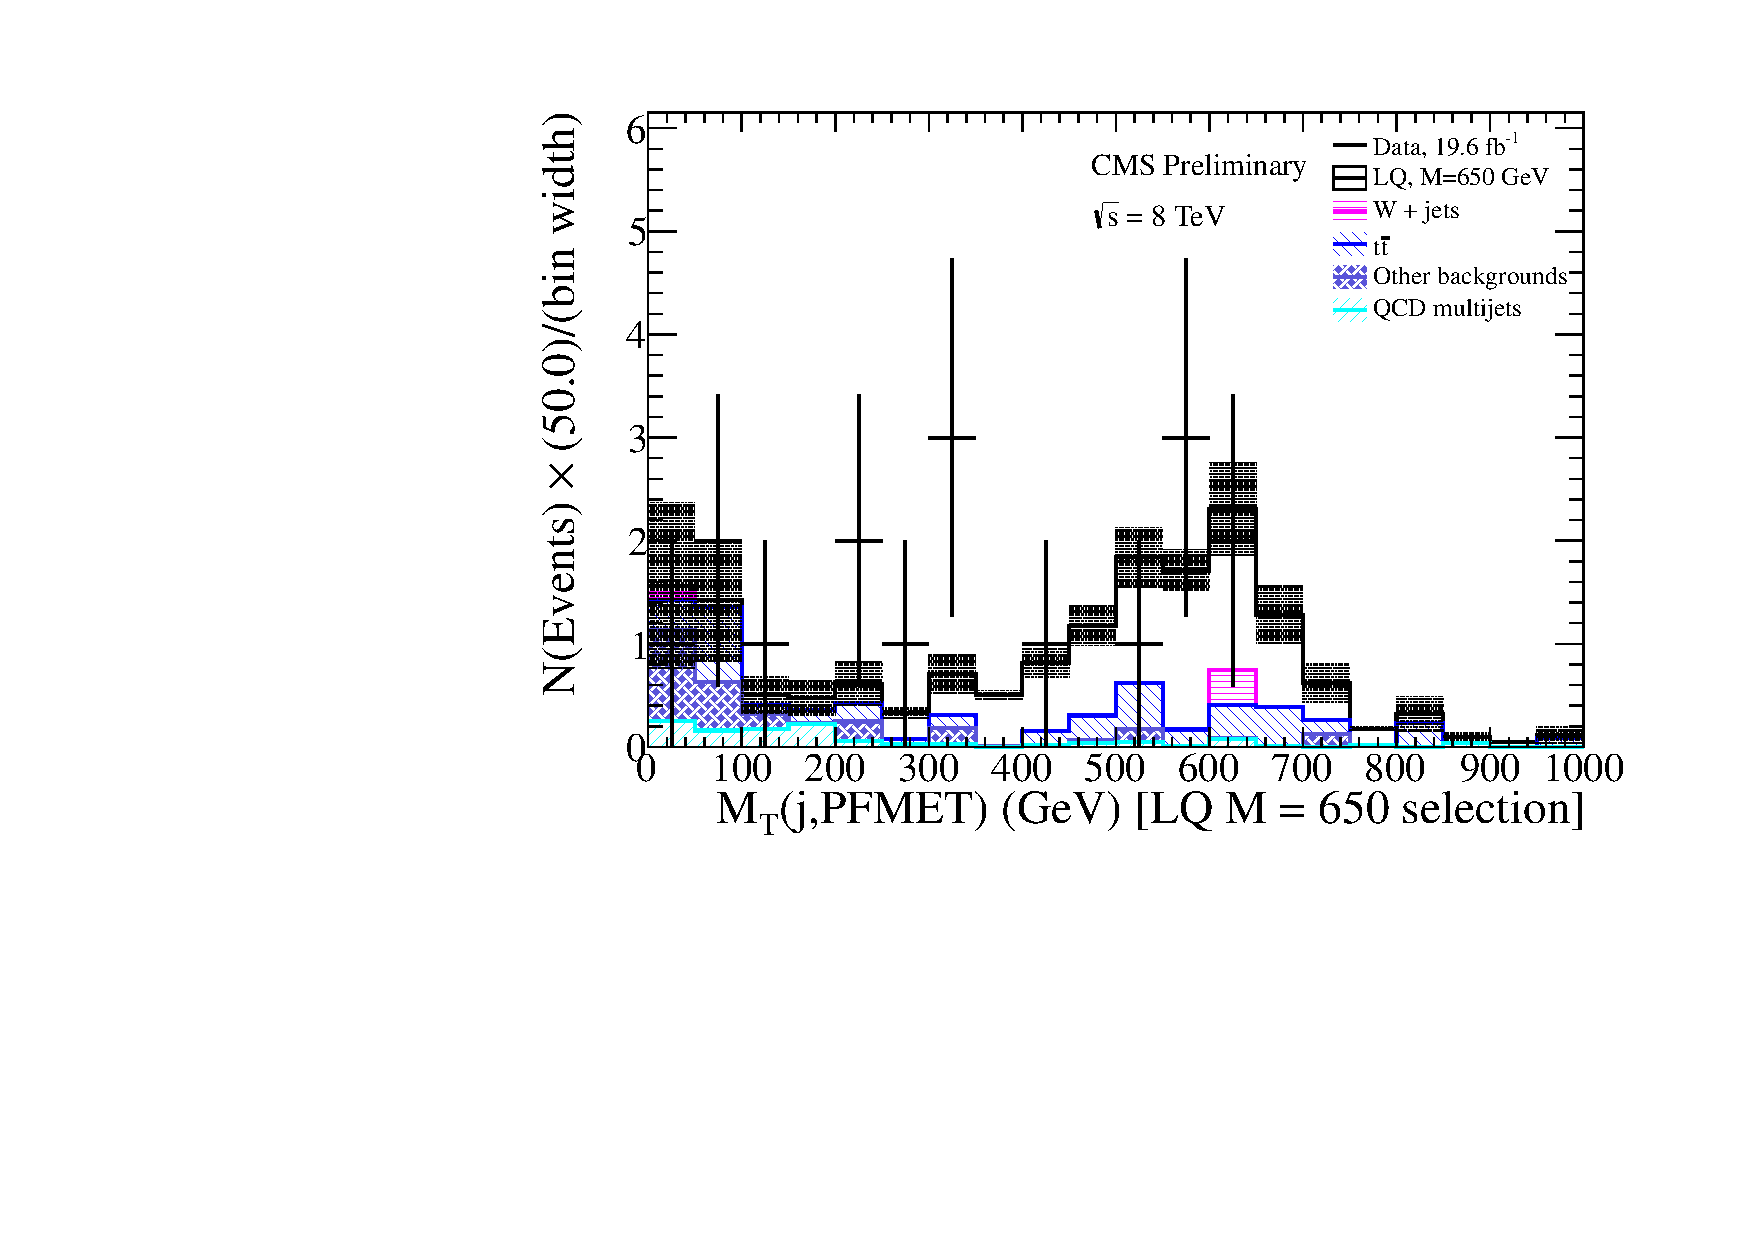
\includegraphics[width=\textwidth]{fig/enu/finalSelection015/MTjnu_LQ650_enujj.pdf}
\end{column}
\end{columns}
\end{frame}
\subsection{Overview of checks}
\label{sec-7-3}
\begin{frame}
\frametitle{Overview of checks}
\label{sec-7-3-1}

\tiny
\begin{itemize}
\item \textbf{Problem with analysis code?} \alert{No} \\ 
$\text{W}_{\text{R}}$ analysis (\eejj final state) reproduced the excess (J. Pastika, B. Dahmes)
\item \textbf{Problem with ECAL?} \alert{No} \\
ECAL DPG says these events are ok.  Electrons are spread in $\eta$ and $\phi$.
\item \textbf{Problem with unstable running conditions?} \alert{No} \\ 
Excesses are flat vs run period.
\item \textbf{Problem with signal trigger?} \alert{No} \\ 
\eejj excess persists with ${\tt HLT\_DoubleEle33\_CaolIdL\_GsfTrkIdVL}$.
\item \textbf{Problem with single object mis-measurement (eejj analysis only)?} \alert{No} \\ 
Events in \eejj excess do not have an excess of single objects (electrons, jets) aligned with \met.
\item \textbf{Problem modeling \met and \mt (\enujj analysis only)?} \alert{...} \\
Discrepancy between data and MC in \met and \mt distributions at \enujj preselection, but reweighting
\mt and \met at preselection increases the final selection discrepancy.
\item \textbf{Problem with electrons from pileup?} \alert{No} \\ 
Electrons in excess have low $d_{Z}$ w.r.t. primary vertex
\item \textbf{Problem with data-driven \ttbar background estimate?} \alert{No} \\
Results with $\ttbar \rightarrow \eejj$ MC agree within statistics
\item \textbf{Problem with your data-driven QCD background estimate?} \alert{No} \\
Excess is almost entirely OS electron pairs.  Contribution from QCD is predicted to be << 1 event.
\item \textbf{Problem with your various MC background estimates?} \alert{No} \\
Background for final selection optimized for $M_{LQ} = 650$ GeV is cross-checked using only data.
\end{itemize}
\end{frame}

\end{document}
